%% ============================================================
%%  compare_equipo_06 — Algorithm Comparison (Problem Set 2, Equipo 06)
%%  Compilar: pdflatex compare_equipo_06.tex (dos pasadas).
%%  Con notas: pdflatex -jobname=compare_equipo_06_notas "\def\connotas{}%% ============================================================
%%  compare_equipo_06 — Algorithm Comparison (Problem Set 2, Equipo 06)
%%  Compilar: pdflatex compare_equipo_06.tex (dos pasadas).
%%  Con notas: pdflatex -jobname=compare_equipo_06_notas "\def\connotas{}%% ============================================================
%%  compare_equipo_06 — Algorithm Comparison (Problem Set 2, Equipo 06)
%%  Compilar: pdflatex compare_equipo_06.tex (dos pasadas).
%%  Con notas: pdflatex -jobname=compare_equipo_06_notas "\def\connotas{}%% ============================================================
%%  compare_equipo_06 — Algorithm Comparison (Problem Set 2, Equipo 06)
%%  Compilar: pdflatex compare_equipo_06.tex (dos pasadas).
%%  Con notas: pdflatex -jobname=compare_equipo_06_notas "\def\connotas{}\input{compare_equipo_06}"
%% ============================================================
\documentclass[aspectratio=169,11pt]{beamer}
\input{preamble}
\input{comun}

\title[Predicting Poverty: Algorithm Comparison]{Predicting Poverty: Algorithm Comparison}
\author[Labastidas y Garcia | Equipo 06]{Esteban David Labastidas Martínez \and Neislen Stiven Garcia Silva}
\institute{Facultad de Economía\\ Universidad de los Andes}
\date[Oct 2026]{Bogotá, octubre de 2026}

\begin{document}
\andessectionslidesfalse

%% 1. Best Model Overview (obligatoria)
\diapositivaoverview

%% ============================================================
\section{Datos}
%% ============================================================
\begin{frame}{La pobreza responde a umbrales e interacciones: terreno favorable para los árboles}
  \begin{columns}[c]
    \column{0.60\textwidth}
      \includegraphics[width=\linewidth]{correlatos_pobreza}
    \column{0.38\textwidth}
      \footnotesize
      \textbf{Intuición.} Un modelo lineal suma efectos; un árbol corta en umbrales y
      combina variables.
      \begin{itemize}
        \item \textbf{No linealidad:} con más ocupados la pobreza sube de 29\,\% a 39\,\% y
          luego cae a 5\,\%.
        \item \textbf{Interacción:} el arriendo pesa distinto si la vivienda es propia o
          arrendada (la interacción más fuerte en un EBM).
        \item \textbf{Desbalance:} 20\,\% de pobres; el umbral se elige fuera de fold.
      \end{itemize}
  \end{columns}
  \takeaway{Esperamos que los métodos de árboles con muchas variables ganen a los lineales.}
  \fuente{Fuente: base de hogares de train (scripts/13\_figuras\_presentacion.R); views/tablas/nivel7/etapa15\_ebm\_importancia.csv.}
  \note{
    \textbf{Qué decir.} Antes de comparar, una predicción desde los datos. La pobreza no
    responde de forma lineal: con cero ocupados es menor que con un tercio, porque hay
    pensionados. Y las variables interactúan: pagar arriendo no significa lo mismo en una
    casa propia que en una arrendada. Eso favorece a los árboles, que cortan en umbrales y
    combinan variables sin que se las especifiquemos.\\[3pt]
    \textbf{Pregunta difícil: ¿no basta con interacciones en el Logit?} Se podrían
    agregar, pero habría que elegirlas a mano entre más de mil pares posibles; los árboles
    las buscan solos. El costo es la interpretabilidad.
  }
\end{frame}

%% ============================================================
\section{Comparación de algoritmos}
%% ============================================================
\begin{frame}{Cancha nivelada: mismas 48 variables, misma receta y misma validación}
  \centering\scriptsize\renewcommand{\arraystretch}{1.12}
  \begin{tabular}{@{}lllr@{}}
    \toprule
    Algoritmo & Búsqueda (validación cruzada de 5 folds) & Elegido & Configs. \\
    \midrule
    LPM y Logit & sin hiperparámetros & & 1 \\
    Elastic Net & grilla: penalización $10^{[-5,\,0]}$ $\times$ mezcla L1/L2 [0, 1] & 0,0002; 0,2 & 120 \\
    CART & grilla: complejidad $10^{[-5,\,-1]}$ $\times$ profundidad [3, 15] & $6\times10^{-5}$; 10 & 36 \\
    Naive Bayes & grilla: suavizado [0,5; 1,5] $\times$ Laplace [0, 3] & 0,5; 0 & 16 \\
    Random Forest & hipercubo: variables por corte [3, 25] $\times$ tamaño de hoja [5, 60] & 23; 24 & 15 \\
    XGBoost & hipercubo: árboles [200, 1000] $\times$ profundidad [3, 8] $\times$ tasa $10^{[-3,\,-1]}$ & 781; 6; 0,020 & 20 \\
    LightGBM & hipercubo de 7 hiperparámetros & ver apéndice & 50 \\
    \bottomrule
  \end{tabular}
  \vspace{0.25cm}

  \raggedright\small
  Todos usan la misma receta (imputación, dummies y escalado ajustados dentro de cada
  fold), el umbral elegido con predicciones fuera de fold y el mismo holdout del 20\,\%.
  \takeaway{Las diferencias de F1 reflejan el algoritmo, no los datos que recibe.}
  \fuente{Fuente: views/tablas/leaderboard\_interno.csv (columnas busqueda e hiperparametros).}
  \note{
    \textbf{Qué decir.} Para que la comparación sea justa, todos los algoritmos reciben
    las mismas 48 variables, el mismo preprocesamiento ajustado solo con los datos de
    entrenamiento de cada fold, y eligen hiperparámetros con validación cruzada de 5 folds.
    Grilla regular cuando hay 1 o 2 hiperparámetros, hipercubo latino cuando hay más.\\[3pt]
    \textbf{Pregunta difícil: ¿no tienen ventaja los que recibieron más configuraciones?}
    LightGBM probó 50 y XGBoost 20, pero XGBoost ya llegaba a 0,746 frente a 0,749: la
    ventaja de tuning es de 0,003. Elastic Net probó 120 y empata con el Logit sin tuning.
  }
\end{frame}

\begin{frame}{Con las mismas variables, el boosting gana y Naive Bayes queda 11 puntos atrás}
  \begin{columns}[c]
    \column{0.60\textwidth}
      \centering\scriptsize\renewcommand{\arraystretch}{1.1}
      \begin{tabular}{@{}lcccc@{}}
        \toprule
        Algoritmo & F1 CV & F1 holdout & Filtración & Subcob. \\
        \midrule
        \textbf{Boosting (LightGBM)} & \textbf{0,744} & \textbf{0,749} & 29,3\,\% & 20,4\,\% \\
        Boosting (XGBoost) & 0,740 & 0,746 & 29,6\,\% & 20,6\,\% \\
        Random Forest & 0,726 & 0,734 & 32,0\,\% & 20,2\,\% \\
        Elastic Net & 0,717 & 0,718 & 33,2\,\% & 22,4\,\% \\
        Logit & 0,717 & 0,718 & 32,7\,\% & 23,2\,\% \\
        CART & 0,697 & 0,701 & 34,3\,\% & 24,8\,\% \\
        LPM & 0,690 & 0,691 & 34,9\,\% & 26,3\,\% \\
        Naive Bayes & 0,643 & 0,640 & 44,0\,\% & 25,2\,\% \\
        \bottomrule
      \end{tabular}
    \column{0.38\textwidth}
      \footnotesize
      \textbf{Filtración} $=$ no pobres entre los atendidos ($1-$precisión).
      \textbf{Subcobertura} $=$ pobres excluidos ($1-$recall).
      \begin{itemize}
        \item El orden se repite en CV y en holdout: no es ruido de una partición.
        \item Los mejores ganan sobre todo en filtración.
        \item Naive Bayes supone variables independientes; aquí están muy correlacionadas.
      \end{itemize}
  \end{columns}
  \takeaway{Los dos más cercanos al ganador son Random Forest y Elastic Net (con Logit).}
  \fuente{Holdout de 32.993 hogares; umbral elegido con OOF. Fuente: views/tablas/comparacion\_algoritmos.csv; views/tablas/leaderboard\_interno.csv.}
  \note{
    \textbf{Qué decir.} Esta es la comparación de los siete algoritmos del curso con las
    mismas variables. El boosting queda primero y Naive Bayes último. El orden es el mismo
    en validación cruzada y en holdout. Los dos contendores más cercanos son Random Forest
    y Elastic Net, que empata con el Logit.\\[3pt]
    \textbf{Pregunta difícil: ¿son significativas estas diferencias?} Con 32.993 hogares,
    el efecto mínimo detectable en holdout está entre 0,0025 y 0,006 según el par: las
    brechas de 0,015 o más están claramente por encima; la de XGBoost frente a LightGBM, no.
  }
\end{frame}

\begin{frame}{Random Forest cubre igual que el boosting, pero filtra más}
  \begin{columns}[T]
    \column{0.50\textwidth}
      \centering\footnotesize
      \begin{tabular}{@{}lcc@{}}
        \toprule
        Holdout, 48 variables & Random Forest & XGBoost \\
        \midrule
        Recall (cobertura) & 0,798 & 0,794 \\
        Precisión & 0,680 & 0,704 \\
        No pobres incluidos & 2.483 & 2.206 \\
        Pobres excluidos & 1.332 & 1.358 \\
        F1 & 0,734 & 0,746 \\
        \bottomrule
      \end{tabular}
      \vspace{0.25cm}

      \begin{tabular}{@{}lcc@{}}
        \toprule
        Con variables de ingreso & F1 holdout & Brecha \\
        \midrule
        LightGBM (todas) & 0,781 & \\
        Random Forest (60 mejores) & 0,776 & $-0{,}005$ \\
        \bottomrule
      \end{tabular}
    \column{0.46\textwidth}
      \footnotesize
      \textbf{Intuición.} Random Forest promedia árboles profundos que aprenden lo mismo en
      paralelo; el boosting suma árboles pequeños que corrigen los errores de los
      anteriores, como los hogares cerca de la línea.
      \begin{itemize}
        \item Misma cobertura, pero 277 no pobres más incluidos: la brecha está en la
          precisión.
        \item Con las variables de ingreso la brecha baja de 0,012 a 0,005: con mejores
          variables, el algoritmo importa menos.
      \end{itemize}
  \end{columns}
  \takeaway{La ventaja del boosting está en la precisión: incluye menos no pobres.}
  \fuente{Fuente: views/tablas/leaderboard\_interno.csv; views/tablas/nivel7/etapa9\_candidatos.csv (Random Forest con las 60 variables de un algoritmo genético; no es cancha nivelada).}
  \note{
    \textbf{Qué decir.} Random Forest es el contendor más cercano. Cubre a los mismos
    pobres que el boosting, pero incluye 277 no pobres más. Una lectura: el bosque promedia
    árboles independientes, mientras el boosting agrega árboles enfocados en los errores
    que quedan, que están cerca de la línea. Con las variables de ingreso, la brecha se
    reduce a la mitad.\\[3pt]
    \textbf{Pregunta difícil: ¿la comparación del nivel 7 es justa?} No del todo: el bosque
    usó 60 variables y LightGBM todas. Por eso solo la usamos para mostrar que la brecha
    se achica, no para medirla.
  }
\end{frame}

\begin{frame}{Elastic Net empata con el Logit: la brecha con el boosting es por la linealidad}
  \begin{columns}[T]
    \column{0.48\textwidth}
      \footnotesize
      \textbf{Intuición.} Elastic Net penaliza coeficientes para evitar el sobreajuste. Con
      131.967 hogares y 48 variables no hay sobreajuste que evitar.
      \begin{itemize}
        \item La validación cruzada elige una penalización casi nula (0,0002).
        \item Mismo F1 en holdout que el Logit: 0,718.
        \item LPM (probabilidad lineal): 0,691, es decir 0,027 menos que el Logit.
      \end{itemize}
    \column{0.48\textwidth}
      \footnotesize
      \textbf{Lo que cuesta la linealidad frente al boosting}
      \begin{itemize}
        \item F1: 0,718 frente a 0,749 ($-0{,}031$).
        \item Subcobertura 22,4\,\% frente a 20,4\,\%: unos 130 pobres más excluidos en
          el holdout.
        \item A cambio, cada coeficiente se puede leer y auditar.
      \end{itemize}
  \end{columns}
  \takeaway{Regularizar no ayuda con muchos datos; lo que falta son umbrales e interacciones.}
  \fuente{Fuente: views/tablas/leaderboard\_interno.csv (n4\_elastic\_net, n3\_logit, n3\_lpm, n6\_lightgbm).}
  \note{
    \textbf{Qué decir.} El segundo contendor es Elastic Net. La validación cruzada elige
    casi no penalizar, porque con más de 130 mil hogares y 48 variables no hay sobreajuste.
    Por eso empata con el Logit. Lo que lo separa del boosting no es la regularización sino
    la forma funcional: no capta umbrales ni interacciones.\\[3pt]
    \textbf{Pregunta difícil: ¿cuántos pobres más excluye?} Con 6.605 pobres en el
    holdout, 2 puntos de subcobertura son unos 130 hogares (1.478 frente a 1.347
    excluidos).
  }
\end{frame}

\begin{frame}{Balancear las clases no mejora: solo mueve el umbral}
  \begin{columns}[c]
    \column{0.50\textwidth}
      \centering\footnotesize
      \begin{tabular}{@{}lcc@{}}
        \toprule
        XGBoost, 48 variables & F1 holdout & Umbral óptimo \\
        \midrule
        Sin balancear & 0,746 & 0,36 \\
        SMOTE & 0,745 & 0,34 \\
        Pesos de clase & 0,744 & 0,66 \\
        Submuestreo & 0,747 & 0,69 \\
        \bottomrule
      \end{tabular}
    \column{0.46\textwidth}
      \footnotesize
      \textbf{Intuición.} Balancear infla la probabilidad de ser pobre. Si después se elige
      el umbral que maximiza F1, ese umbral sube y deshace el cambio.
      \begin{itemize}
        \item Diferencias de F1 de 0,002 o menos, dentro del ruido.
        \item El umbral pasa de 0,36 a 0,66--0,69 con pesos o submuestreo.
      \end{itemize}
  \end{columns}
  \takeaway{Con el umbral elegido fuera de fold, el desbalance ya está resuelto.}
  \fuente{Fuente: views/tablas/leaderboard\_interno.csv (n4\_xgboost y n5\_*).}
  \note{
    \textbf{Qué decir.} Probamos las tres estrategias clásicas sobre el mejor algoritmo
    de ese nivel. Ninguna cambia el F1 más allá de 0,002. Lo que sí cambia es el umbral
    óptimo, porque el balanceo solo reescala las probabilidades.\\[3pt]
    \textbf{Pregunta difícil: ¿y si no se eligiera el umbral?} Con el umbral fijo en 0,5,
    esperaríamos que balancear sí ayudara, porque acerca las probabilidades al punto de
    corte (no lo medimos). Elegir el umbral es la forma directa de lograr lo mismo.
  }
\end{frame}

\begin{frame}{Cambiar las variables vale 9 veces más que cambiar el algoritmo}
  \begin{columns}[c]
    \column{0.66\textwidth}
      \includegraphics[width=\linewidth]{escalera_completa}
    \column{0.32\textwidth}
      \footnotesize
      \textbf{Suma de los saltos}
      \begin{itemize}
        \item \textcolor{andesaccent}{\textbf{Variables}}: $+0{,}292$.
        \item \textbf{Algoritmo}: $+0{,}032$.
      \end{itemize}
      La variable que más aportó predice el ingreso de cada persona con un modelo
      auxiliar y lo suma al hogar.
  \end{columns}
  \takeaway{La mejor inversión fue entender el hogar, no elegir el algoritmo.}
  \fuente{F1 en holdout. Fuente: views/tablas/leaderboard\_interno.csv y nivel7/ (ablacion\_etapa1, resumen\_etapa2, etapa6\_ablacion, etapa7\_a, etapa18\_resumen).}
  \note{
    \textbf{Qué decir.} Poniendo la comparación en perspectiva: toda la diferencia entre
    algoritmos que acabamos de ver suma 0,03 de F1. Construir variables desde las
    personas, y sobre todo predecir el ingreso de cada persona, sumó 0,29.\\[3pt]
    \textbf{Pregunta difícil: ¿no depende del orden de los pasos?} Sí, la descomposición
    es secuencial. Pero en cualquier orden el contraste es grande: con LightGBM fijo las
    variables nuevas suman 0,032, más que toda la diferencia entre Logit y boosting.
  }
\end{frame}

\begin{frame}{Con las variables de ingreso, todos los algoritmos convergen}
  \begin{columns}[c]
    \column{0.55\textwidth}
      \centering\scriptsize\renewcommand{\arraystretch}{1.1}
      \begin{tabular}{@{}lcc@{}}
        \toprule
        Base de 1.324 variables & F1 holdout & Corr.\ OOF \\
        \midrule
        \textbf{LightGBM} & \textbf{0,781} & 1 \\
        CatBoost & 0,779 & 0,994 \\
        AutoGluon (AutoML) & 0,777 & 0,990 \\
        RealMLP (red neuronal) & 0,775 & 0,984 \\
        TabM (red neuronal) & 0,767 & 0,977 \\
        \bottomrule
      \end{tabular}
    \column{0.43\textwidth}
      \footnotesize
      \textbf{Intuición.} Si todos predicen casi lo mismo, la información se agotó en las
      variables.
      \begin{itemize}
        \item Corr.\ OOF: correlación de sus predicciones fuera de fold con las de LightGBM; entre 0,98 y 0,99.
        \item AutoGluon sobre la base cruda, sin nuestras variables: 0,763.
        \item Mezclar los mejores suma una milésima (0,782).
      \end{itemize}
  \end{columns}
  \takeaway{El techo es común a todos: es de información, no de algoritmo.}
  \fuente{Fuente: views/tablas/nivel7/etapa7\_b.csv, etapa10\_candidatos.csv, etapa12\_resumen.csv, etapa18\_resumen.csv.}
  \note{
    \textbf{Qué decir.} Fuera de la lista del curso probamos CatBoost, redes neuronales
    tabulares y AutoML. Con nuestras variables todos quedan a menos de 0,015 de LightGBM y
    sus predicciones son casi idénticas. AutoGluon con la base cruda pierde 1,7 puntos: lo
    que le falta son nuestras variables, no capacidad de modelar.\\[3pt]
    \textbf{Pregunta difícil: ¿por qué gana LightGBM y no la red?} Con datos tabulares de
    este tamaño, los árboles con boosting suelen ganar a las redes; aquí la diferencia es de
    0,005, del orden del efecto mínimo detectable.
  }
\end{frame}

%% ============================================================
\section{Conclusión}
%% ============================================================
\begin{frame}{Más complejidad compra 6 puntos de F1 y protege más a los más pobres}
  \centering\footnotesize\renewcommand{\arraystretch}{1.12}
  \begin{tabular}{@{}lccc@{}}
    \toprule
    & Encuesta corta (Logit) & Logit completo & Mejor modelo \\
    \midrule
    Variables & 8 & 48 & 1.324 + auxiliares \\
    F1 holdout & 0,664 & 0,718 & 0,782 \\
    Subcobertura & 26,0\,\% & 23,2\,\% & 18,2\,\% \\
    Filtración & 39,8\,\% & 32,7\,\% & 25,1\,\% \\
    Excluidos en pobreza extrema & 16,1\,\% & 14,8\,\% & 11,2\,\% \\
    Interpretación & coeficientes & coeficientes & importancia y curvas \\
    Costo de recolección & bajo & medio & alto (módulo laboral) \\
    \bottomrule
  \end{tabular}
  \vspace{0.2cm}

  \raggedright\footnotesize
  Pobreza extrema: ingreso menor a la mitad de la línea, como porcentaje de los pobres excluidos.
  \takeaway{La complejidad se justifica por a quién deja de excluir, no por el F1 en sí.}
  \fuente{Holdout, umbral elegido con OOF. Fuente: views/tablas/nivel7/etapa15\_pesos\_bienestar.csv (mejor modelo: mezcla sin el modelo limpio).}
  \note{
    \textbf{Qué decir.} El trade-off concreto: pasar de 8 preguntas a un Logit completo y
    luego al mejor modelo baja la subcobertura de 26 a 18\,\% y la filtración de 40 a
    25\,\%. Y no solo excluye menos: los que excluye están más cerca de la línea.\\[3pt]
    \textbf{Pregunta difícil: ¿el mejor modelo es interpretable?} No como un Logit, pero
    sus decisiones se explican con dos cosas: ingreso predicho y vivienda. Un EBM llega a
    0,777 con curvas legibles, por si la agencia exige transparencia.
  }
\end{frame}

\begin{frame}{¿El modelo con más score en Kaggle? No necesariamente}
  \small
  \textbf{Lo que recomendaríamos a una agencia}
  \begin{enumerate}
    \item \textbf{Elegir por el costo de los errores, no por F1:} el F1 supone que excluir y
      filtrar cuestan igual; una agencia puede preferir más cobertura.
    \item \textbf{LightGBM solo, no la mezcla:} rinde igual (diferencia de milésimas) y es más
      simple de mantener y auditar.
    \item \textbf{Si exige transparencia:} un EBM (0,777) o un Logit (0,718) con el mismo
      módulo laboral, aceptando más subcobertura.
    \item \textbf{Si solo hay encuesta corta:} el Logit de 8 preguntas como filtro, con un
      umbral más bajo y verificación posterior.
  \end{enumerate}
  \takeaway{La mejor decisión depende de qué se puede medir y de cuánto cuesta excluir a un pobre.}
  \fuente{Fuente: views/tablas/nivel7/etapa15\_resumen.csv (EBM); views/tablas/leaderboard\_interno.csv; views/tablas/nivel7/etapa18\_resumen.csv.}
  \note{
    \textbf{Qué decir.} No necesariamente el de mayor Kaggle. La diferencia entre la
    mezcla y LightGBM solo es de milésimas, así que recomendamos el más simple. Si la
    agencia necesita explicar cada decisión, un EBM pierde medio punto. Y si solo puede
    pagar una encuesta corta, debe compensar con un umbral más bajo y verificación.\\[3pt]
    \textbf{Pregunta difícil: ¿por qué no recomiendan directamente el Logit, que es
    transparente?} Porque excluye a 5 puntos más de pobres y más de ellos en pobreza
    extrema; esa es una pérdida de bienestar que hay que poner en la balanza.
  }
\end{frame}

%% ============================================================
%% Apéndice
%% ============================================================
\appendix
\diapositivaglosario

\begin{frame}{Apéndice: hiperparámetros del LightGBM ganador}
  \centering\footnotesize\renewcommand{\arraystretch}{1.12}
  \begin{tabular}{@{}llll@{}}
    \toprule
    Hiperparámetro & Rango explorado & Elegido & Lectura \\
    \midrule
    Número de árboles & [200, 2000] & 1.852 & muchos árboles \\
    Tasa de aprendizaje & $10^{[-3,\,-0{,}7]}$ & 0,011 & pasos pequeños \\
    Profundidad máxima & [3, 12] & 12 (31 hojas) & árboles medianos \\
    Mínimo de hogares por hoja & [10, 200] & 171 & no memoriza casos \\
    Variables por corte & [0,2; 1] & 0,82 & algo de azar \\
    Hogares por árbol & [0,5; 1] & 0,70 & algo de azar \\
    Ganancia mínima para cortar & $10^{[-10,\,1]}$ & $7\times10^{-10}$ & sin restricción \\
    \bottomrule
  \end{tabular}
  \fuente{Hipercubo latino de 50 configuraciones, validación cruzada de 5 folds sobre las 48 variables. Fuente: views/tablas/leaderboard\_interno.csv (n6\_lightgbm).}
  \note{Respaldo: la configuración que se reutilizó en todo el nivel 7.}
\end{frame}

\begin{frame}{Apéndice: en CV repetida ninguna alternativa mejora de forma detectable}
  \centering\scriptsize
  \begin{tabular}{@{}lccc@{}}
    \toprule
    Candidato & F1 CV repetida (EE) & $\Delta$ vs.\ LightGBM [IC 95\,\%] & F1 holdout [IC 95\,\%] \\
    \midrule
    LightGBM base & 0,7752 (0,0008) & & 0,7806 [0,7731; 0,7885] \\
    + redes (mezcla sin limpio) & 0,7758 (0,0008) & $+0{,}0006$ [$-0{,}0001$; $+0{,}0013$] & 0,7820 [0,7743; 0,7897] \\
    \textbf{+ redes + limpio (final)} & \textbf{0,7759 (0,0008)} & $+0{,}0007$ [$+0{,}0002$; $+0{,}0012$] & 0,7817 [0,7742; 0,7894] \\
    CatBoost & 0,7722 (0,0007) & $-0{,}0030$ [$-0{,}0042$; $-0{,}0018$] & 0,7786 [0,7707; 0,7864] \\
    Rediseño desde cero & 0,7478 (0,0008) & $-0{,}0274$ [$-0{,}0289$; $-0{,}0260$] & 0,7499 [0,7420; 0,7581] \\
    \bottomrule
  \end{tabular}
  \fuente{IC pareados ingenuos (15 pares). Con la corrección de Nadeau y Bengio el IC del modelo final es [$-0{,}0004$; $+0{,}0017$]. Fuente: views/tablas/nivel7/etapa16\_fase1\_resumen.csv, etapa18\_resumen.csv.}
  \note{Respaldo: CatBoost pierde con un IC que excluye cero; la mezcla gana por milésimas.}
\end{frame}

\end{document}
"
%% ============================================================
\documentclass[aspectratio=169,11pt]{beamer}
%% Preamble: packages and theme. Keep design changes in beamerthemeUniandes.sty
\usepackage[utf8]{inputenc}
\usepackage[T1]{fontenc}
\usepackage[spanish,es-nodecimaldot,es-noshorthands]{babel}
\usepackage{amsmath,amssymb}
\usepackage{graphicx}
\usepackage{booktabs}
\usepackage[round]{natbib}
\usetheme{Uniandes}

%% ---- Agregados para el Problem Set 2 (no cambian el diseño) ----
% Algunas instalaciones de MiKTeX no registran el mapa de Source Sans; se carga aquí.
\pdfmapfile{+SourceSansThree.map}
\usepackage{array}
\usepackage{xspace}
\usetikzlibrary{positioning,arrows.meta,decorations.pathreplacing}
\graphicspath{{../figuras/}{../../../views/figuras/}{../../../views/figuras/nivel7/}}

% Notas del presentador: el PDF de entrega no las muestra; la versión *_notas
% se compila con \def\connotas{} antes del documento y las intercala.
\ifdefined\connotas
  \setbeameroption{show notes}
\else
  \setbeameroption{hide notes}
\fi
\setbeamerfont{note page}{size=\small}
\setbeamertemplate{note page}{%
  \vspace{0.3cm}\insertslideintonotes{0.25}\par\vspace{0.2cm}
  \begin{minipage}{0.95\textwidth}\insertnote\end{minipage}}

% F1 público de Kaggle del mejor modelo (n18), tal como lo muestra la Overview.
\def\kagglepublico{0,78}

% Tabla pequeña con letra reducida
\newcommand{\tablachica}{\footnotesize\renewcommand{\arraystretch}{1.12}}
% Fuente de una figura o tabla, al pie
\newcommand{\fuente}[1]{\par\vspace{2pt}{\tiny\color{andesgray}#1\par}}
% Títulos sin cortar palabras con guion: se hace dentro de la plantilla del título
% (beamerthemeUniandes.sty), porque el minipage del título reinicia la alineación.
% Cajas de los diagramas sin guiones
\tikzset{every node/.append style={execute at begin node={\hyphenpenalty=10000\exhyphenpenalty=10000}}}

%% ============================================================
%%  Piezas comunes a los dos decks: Best Model Overview y glosario
%% ============================================================

% ---- Best Model Overview (diapositiva obligatoria, primera de cada deck) ----
\newcommand{\diapositivaoverview}{%
\begin{frame}{Best Model Overview}
  {Ingreso predicho por persona + LightGBM \;|\; Equipo 06, MECA 4107}
  \vspace{-0.1cm}
  \begin{columns}[T]
    \column{0.37\textwidth}\centering \keyfig{\kagglepublico}{F1 público en Kaggle}
    \column{0.30\textwidth}\centering \keyfig{0,782}{F1 en holdout, IC 95\,\% [0,774; 0,789]}
    \column{0.30\textwidth}\centering \keyfig{0,776}{F1 en CV repetida (15 evaluaciones)}
  \end{columns}
  \vspace{0.15cm}
  \footnotesize
  \begin{columns}[T]
    \column{0.49\textwidth}
      \textbf{Especificación}
      \begin{itemize}
        \item \textbf{Variable clave:} el ingreso de cada persona, predicho con lo que el test
          sí trae y sumado al hogar (1.324 variables en total).
        \item \textbf{Algoritmo:} LightGBM (76\,\%) mezclado con dos redes (19\,\%) y un
          rediseño desde cero (5\,\%); pesos elegidos fuera de muestra.
        \item \textbf{Regla:} pobre si $P(\text{pobre}) \geq 0{,}36$.
      \end{itemize}
    \column{0.49\textwidth}
      \textbf{Mensajes}
      \begin{enumerate}
        \item Las variables aportaron \textbf{9 veces más} F1 que los algoritmos.
        \item El techo (${\approx}\,0{,}78$) viene sobre todo de la información que falta.
        \item Excluye al 18\,\% de los pobres, casi todos cerca de la línea.
      \end{enumerate}
  \end{columns}
  \fuente{F1: media armónica de precisión y recall de la clase pobre. Holdout: 20\,\% del train nunca usado para decidir. Fuente: views/tablas/nivel7/etapa18\_resumen.csv.}
  \note{
    \textbf{Qué decir (1 min).} Nuestro mejor modelo clasifica hogares pobres con F1 de
    0,782 en datos que nunca usamos para decidir. La pieza clave no es el algoritmo sino
    una variable: predecimos cuánto gana cada persona con lo que el test sí trae
    (ocupación, horas, cotización) y lo sumamos al hogar. Tres mensajes: las variables
    pesan 9 veces más que el algoritmo, hay un techo que viene de los datos y los errores
    se concentran cerca de la línea.\\[3pt]
    \textbf{Pregunta difícil: ¿por qué una mezcla y no un solo modelo?} La mezcla gana
    +0,0007 en CV repetida frente a LightGBM solo. El IC ingenuo [+0,0002; +0,0012] excluye
    cero; el corregido por dependencia entre folds no. Es una mejora marginal: en la
    práctica LightGBM solo rinde igual.
  }
\end{frame}}

% ---- Glosario (apéndice de ambos decks, dos diapositivas) ----
\newcommand{\filaglosario}[2]{\textbf{#1} & #2 \\}
\newcommand{\diapositivaglosario}{%
\begin{frame}{Glosario (1/2): métricas y errores}
  \footnotesize\renewcommand{\arraystretch}{1.25}
  \begin{tabular}{@{}p{0.2\textwidth}p{0.76\textwidth}@{}}
    \toprule
    \filaglosario{Precisión}{De los hogares que el programa atiende, qué parte es pobre. $1-$precisión $=$ \textbf{filtración}: no pobres que reciben el beneficio.}
    \filaglosario{Recall}{De los hogares pobres, qué parte atiende el programa. $1-$recall $=$ \textbf{subcobertura}: pobres excluidos.}
    \filaglosario{F1}{Media armónica de precisión y recall: solo es alta si ambas lo son. No premia a los no pobres bien clasificados.}
    \filaglosario{Umbral}{Probabilidad a partir de la cual un hogar se clasifica como pobre. Bajarlo cubre más pobres a cambio de más filtración.}
    \filaglosario{IC 95\,\%}{Rango de valores compatibles con los datos. Si el IC de una diferencia incluye cero, no podemos afirmar que haya mejora.}
    \filaglosario{Efecto mínimo detectable}{La mejora más pequeña que el diseño detectaría con probabilidad 0,8.}
    \bottomrule
  \end{tabular}
  \note{Glosario de apoyo; se muestra solo si lo preguntan.}
\end{frame}
\begin{frame}{Glosario (2/2): validación y variables}
  \footnotesize\renewcommand{\arraystretch}{1.25}
  \begin{tabular}{@{}p{0.2\textwidth}p{0.76\textwidth}@{}}
    \toprule
    \filaglosario{Holdout}{20\,\% del train (32.993 hogares) apartado al inicio; solo se usa para medir, nunca para decidir.}
    \filaglosario{Validación cruzada}{El 80\,\% restante se parte en 5 bloques (folds): se entrena con 4 y se evalúa en el quinto, rotando.}
    \filaglosario{Fuera de fold (OOF)}{La predicción de cada hogar hecha por un modelo que no lo vio. Con ella se eligen umbral, pesos e hiperparámetros.}
    \filaglosario{CV repetida}{La validación cruzada repetida con 3 particiones nuevas: 15 evaluaciones para medir la variabilidad.}
    \filaglosario{Auxiliar de ingreso}{Modelo que predice el ingreso de cada persona con variables que el test sí trae; sumado al hogar, entra como variable.}
    \filaglosario{OOF anidada}{El auxiliar que alimenta a un hogar no vio ese hogar ni su fold de validación: así no se filtra la respuesta.}
    \bottomrule
  \end{tabular}
  \note{Glosario de apoyo; se muestra solo si lo preguntan.}
\end{frame}}


\title[Predicting Poverty: Algorithm Comparison]{Predicting Poverty: Algorithm Comparison}
\author[Labastidas y Garcia | Equipo 06]{Esteban David Labastidas Martínez \and Neislen Stiven Garcia Silva}
\institute{Facultad de Economía\\ Universidad de los Andes}
\date[Oct 2026]{Bogotá, octubre de 2026}

\begin{document}
\andessectionslidesfalse

%% 1. Best Model Overview (obligatoria)
\diapositivaoverview

%% ============================================================
\section{Datos}
%% ============================================================
\begin{frame}{La pobreza responde a umbrales e interacciones: terreno favorable para los árboles}
  \begin{columns}[c]
    \column{0.60\textwidth}
      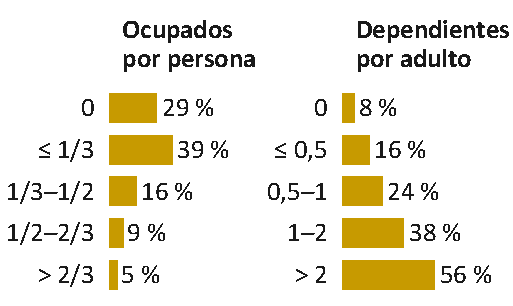
\includegraphics[width=\linewidth]{correlatos_pobreza}
    \column{0.38\textwidth}
      \footnotesize
      \textbf{Intuición.} Un modelo lineal suma efectos; un árbol corta en umbrales y
      combina variables.
      \begin{itemize}
        \item \textbf{No linealidad:} con más ocupados la pobreza sube de 29\,\% a 39\,\% y
          luego cae a 5\,\%.
        \item \textbf{Interacción:} el arriendo pesa distinto si la vivienda es propia o
          arrendada (la interacción más fuerte en un EBM).
        \item \textbf{Desbalance:} 20\,\% de pobres; el umbral se elige fuera de fold.
      \end{itemize}
  \end{columns}
  \takeaway{Esperamos que los métodos de árboles con muchas variables ganen a los lineales.}
  \fuente{Fuente: base de hogares de train (scripts/13\_figuras\_presentacion.R); views/tablas/nivel7/etapa15\_ebm\_importancia.csv.}
  \note{
    \textbf{Qué decir.} Antes de comparar, una predicción desde los datos. La pobreza no
    responde de forma lineal: con cero ocupados es menor que con un tercio, porque hay
    pensionados. Y las variables interactúan: pagar arriendo no significa lo mismo en una
    casa propia que en una arrendada. Eso favorece a los árboles, que cortan en umbrales y
    combinan variables sin que se las especifiquemos.\\[3pt]
    \textbf{Pregunta difícil: ¿no basta con interacciones en el Logit?} Se podrían
    agregar, pero habría que elegirlas a mano entre más de mil pares posibles; los árboles
    las buscan solos. El costo es la interpretabilidad.
  }
\end{frame}

%% ============================================================
\section{Comparación de algoritmos}
%% ============================================================
\begin{frame}{Cancha nivelada: mismas 48 variables, misma receta y misma validación}
  \centering\scriptsize\renewcommand{\arraystretch}{1.12}
  \begin{tabular}{@{}lllr@{}}
    \toprule
    Algoritmo & Búsqueda (validación cruzada de 5 folds) & Elegido & Configs. \\
    \midrule
    LPM y Logit & sin hiperparámetros & & 1 \\
    Elastic Net & grilla: penalización $10^{[-5,\,0]}$ $\times$ mezcla L1/L2 [0, 1] & 0,0002; 0,2 & 120 \\
    CART & grilla: complejidad $10^{[-5,\,-1]}$ $\times$ profundidad [3, 15] & $6\times10^{-5}$; 10 & 36 \\
    Naive Bayes & grilla: suavizado [0,5; 1,5] $\times$ Laplace [0, 3] & 0,5; 0 & 16 \\
    Random Forest & hipercubo: variables por corte [3, 25] $\times$ tamaño de hoja [5, 60] & 23; 24 & 15 \\
    XGBoost & hipercubo: árboles [200, 1000] $\times$ profundidad [3, 8] $\times$ tasa $10^{[-3,\,-1]}$ & 781; 6; 0,020 & 20 \\
    LightGBM & hipercubo de 7 hiperparámetros & ver apéndice & 50 \\
    \bottomrule
  \end{tabular}
  \vspace{0.25cm}

  \raggedright\small
  Todos usan la misma receta (imputación, dummies y escalado ajustados dentro de cada
  fold), el umbral elegido con predicciones fuera de fold y el mismo holdout del 20\,\%.
  \takeaway{Las diferencias de F1 reflejan el algoritmo, no los datos que recibe.}
  \fuente{Fuente: views/tablas/leaderboard\_interno.csv (columnas busqueda e hiperparametros).}
  \note{
    \textbf{Qué decir.} Para que la comparación sea justa, todos los algoritmos reciben
    las mismas 48 variables, el mismo preprocesamiento ajustado solo con los datos de
    entrenamiento de cada fold, y eligen hiperparámetros con validación cruzada de 5 folds.
    Grilla regular cuando hay 1 o 2 hiperparámetros, hipercubo latino cuando hay más.\\[3pt]
    \textbf{Pregunta difícil: ¿no tienen ventaja los que recibieron más configuraciones?}
    LightGBM probó 50 y XGBoost 20, pero XGBoost ya llegaba a 0,746 frente a 0,749: la
    ventaja de tuning es de 0,003. Elastic Net probó 120 y empata con el Logit sin tuning.
  }
\end{frame}

\begin{frame}{Con las mismas variables, el boosting gana y Naive Bayes queda 11 puntos atrás}
  \begin{columns}[c]
    \column{0.60\textwidth}
      \centering\scriptsize\renewcommand{\arraystretch}{1.1}
      \begin{tabular}{@{}lcccc@{}}
        \toprule
        Algoritmo & F1 CV & F1 holdout & Filtración & Subcob. \\
        \midrule
        \textbf{Boosting (LightGBM)} & \textbf{0,744} & \textbf{0,749} & 29,3\,\% & 20,4\,\% \\
        Boosting (XGBoost) & 0,740 & 0,746 & 29,6\,\% & 20,6\,\% \\
        Random Forest & 0,726 & 0,734 & 32,0\,\% & 20,2\,\% \\
        Elastic Net & 0,717 & 0,718 & 33,2\,\% & 22,4\,\% \\
        Logit & 0,717 & 0,718 & 32,7\,\% & 23,2\,\% \\
        CART & 0,697 & 0,701 & 34,3\,\% & 24,8\,\% \\
        LPM & 0,690 & 0,691 & 34,9\,\% & 26,3\,\% \\
        Naive Bayes & 0,643 & 0,640 & 44,0\,\% & 25,2\,\% \\
        \bottomrule
      \end{tabular}
    \column{0.38\textwidth}
      \footnotesize
      \textbf{Filtración} $=$ no pobres entre los atendidos ($1-$precisión).
      \textbf{Subcobertura} $=$ pobres excluidos ($1-$recall).
      \begin{itemize}
        \item El orden se repite en CV y en holdout: no es ruido de una partición.
        \item Los mejores ganan sobre todo en filtración.
        \item Naive Bayes supone variables independientes; aquí están muy correlacionadas.
      \end{itemize}
  \end{columns}
  \takeaway{Los dos más cercanos al ganador son Random Forest y Elastic Net (con Logit).}
  \fuente{Holdout de 32.993 hogares; umbral elegido con OOF. Fuente: views/tablas/comparacion\_algoritmos.csv; views/tablas/leaderboard\_interno.csv.}
  \note{
    \textbf{Qué decir.} Esta es la comparación de los siete algoritmos del curso con las
    mismas variables. El boosting queda primero y Naive Bayes último. El orden es el mismo
    en validación cruzada y en holdout. Los dos contendores más cercanos son Random Forest
    y Elastic Net, que empata con el Logit.\\[3pt]
    \textbf{Pregunta difícil: ¿son significativas estas diferencias?} Con 32.993 hogares,
    el efecto mínimo detectable en holdout está entre 0,0025 y 0,006 según el par: las
    brechas de 0,015 o más están claramente por encima; la de XGBoost frente a LightGBM, no.
  }
\end{frame}

\begin{frame}{Random Forest cubre igual que el boosting, pero filtra más}
  \begin{columns}[T]
    \column{0.50\textwidth}
      \centering\footnotesize
      \begin{tabular}{@{}lcc@{}}
        \toprule
        Holdout, 48 variables & Random Forest & XGBoost \\
        \midrule
        Recall (cobertura) & 0,798 & 0,794 \\
        Precisión & 0,680 & 0,704 \\
        No pobres incluidos & 2.483 & 2.206 \\
        Pobres excluidos & 1.332 & 1.358 \\
        F1 & 0,734 & 0,746 \\
        \bottomrule
      \end{tabular}
      \vspace{0.25cm}

      \begin{tabular}{@{}lcc@{}}
        \toprule
        Con variables de ingreso & F1 holdout & Brecha \\
        \midrule
        LightGBM (todas) & 0,781 & \\
        Random Forest (60 mejores) & 0,776 & $-0{,}005$ \\
        \bottomrule
      \end{tabular}
    \column{0.46\textwidth}
      \footnotesize
      \textbf{Intuición.} Random Forest promedia árboles profundos que aprenden lo mismo en
      paralelo; el boosting suma árboles pequeños que corrigen los errores de los
      anteriores, como los hogares cerca de la línea.
      \begin{itemize}
        \item Misma cobertura, pero 277 no pobres más incluidos: la brecha está en la
          precisión.
        \item Con las variables de ingreso la brecha baja de 0,012 a 0,005: con mejores
          variables, el algoritmo importa menos.
      \end{itemize}
  \end{columns}
  \takeaway{La ventaja del boosting está en la precisión: incluye menos no pobres.}
  \fuente{Fuente: views/tablas/leaderboard\_interno.csv; views/tablas/nivel7/etapa9\_candidatos.csv (Random Forest con las 60 variables de un algoritmo genético; no es cancha nivelada).}
  \note{
    \textbf{Qué decir.} Random Forest es el contendor más cercano. Cubre a los mismos
    pobres que el boosting, pero incluye 277 no pobres más. Una lectura: el bosque promedia
    árboles independientes, mientras el boosting agrega árboles enfocados en los errores
    que quedan, que están cerca de la línea. Con las variables de ingreso, la brecha se
    reduce a la mitad.\\[3pt]
    \textbf{Pregunta difícil: ¿la comparación del nivel 7 es justa?} No del todo: el bosque
    usó 60 variables y LightGBM todas. Por eso solo la usamos para mostrar que la brecha
    se achica, no para medirla.
  }
\end{frame}

\begin{frame}{Elastic Net empata con el Logit: la brecha con el boosting es por la linealidad}
  \begin{columns}[T]
    \column{0.48\textwidth}
      \footnotesize
      \textbf{Intuición.} Elastic Net penaliza coeficientes para evitar el sobreajuste. Con
      131.967 hogares y 48 variables no hay sobreajuste que evitar.
      \begin{itemize}
        \item La validación cruzada elige una penalización casi nula (0,0002).
        \item Mismo F1 en holdout que el Logit: 0,718.
        \item LPM (probabilidad lineal): 0,691, es decir 0,027 menos que el Logit.
      \end{itemize}
    \column{0.48\textwidth}
      \footnotesize
      \textbf{Lo que cuesta la linealidad frente al boosting}
      \begin{itemize}
        \item F1: 0,718 frente a 0,749 ($-0{,}031$).
        \item Subcobertura 22,4\,\% frente a 20,4\,\%: unos 130 pobres más excluidos en
          el holdout.
        \item A cambio, cada coeficiente se puede leer y auditar.
      \end{itemize}
  \end{columns}
  \takeaway{Regularizar no ayuda con muchos datos; lo que falta son umbrales e interacciones.}
  \fuente{Fuente: views/tablas/leaderboard\_interno.csv (n4\_elastic\_net, n3\_logit, n3\_lpm, n6\_lightgbm).}
  \note{
    \textbf{Qué decir.} El segundo contendor es Elastic Net. La validación cruzada elige
    casi no penalizar, porque con más de 130 mil hogares y 48 variables no hay sobreajuste.
    Por eso empata con el Logit. Lo que lo separa del boosting no es la regularización sino
    la forma funcional: no capta umbrales ni interacciones.\\[3pt]
    \textbf{Pregunta difícil: ¿cuántos pobres más excluye?} Con 6.605 pobres en el
    holdout, 2 puntos de subcobertura son unos 130 hogares (1.478 frente a 1.347
    excluidos).
  }
\end{frame}

\begin{frame}{Balancear las clases no mejora: solo mueve el umbral}
  \begin{columns}[c]
    \column{0.50\textwidth}
      \centering\footnotesize
      \begin{tabular}{@{}lcc@{}}
        \toprule
        XGBoost, 48 variables & F1 holdout & Umbral óptimo \\
        \midrule
        Sin balancear & 0,746 & 0,36 \\
        SMOTE & 0,745 & 0,34 \\
        Pesos de clase & 0,744 & 0,66 \\
        Submuestreo & 0,747 & 0,69 \\
        \bottomrule
      \end{tabular}
    \column{0.46\textwidth}
      \footnotesize
      \textbf{Intuición.} Balancear infla la probabilidad de ser pobre. Si después se elige
      el umbral que maximiza F1, ese umbral sube y deshace el cambio.
      \begin{itemize}
        \item Diferencias de F1 de 0,002 o menos, dentro del ruido.
        \item El umbral pasa de 0,36 a 0,66--0,69 con pesos o submuestreo.
      \end{itemize}
  \end{columns}
  \takeaway{Con el umbral elegido fuera de fold, el desbalance ya está resuelto.}
  \fuente{Fuente: views/tablas/leaderboard\_interno.csv (n4\_xgboost y n5\_*).}
  \note{
    \textbf{Qué decir.} Probamos las tres estrategias clásicas sobre el mejor algoritmo
    de ese nivel. Ninguna cambia el F1 más allá de 0,002. Lo que sí cambia es el umbral
    óptimo, porque el balanceo solo reescala las probabilidades.\\[3pt]
    \textbf{Pregunta difícil: ¿y si no se eligiera el umbral?} Con el umbral fijo en 0,5,
    esperaríamos que balancear sí ayudara, porque acerca las probabilidades al punto de
    corte (no lo medimos). Elegir el umbral es la forma directa de lograr lo mismo.
  }
\end{frame}

\begin{frame}{Cambiar las variables vale 9 veces más que cambiar el algoritmo}
  \begin{columns}[c]
    \column{0.66\textwidth}
      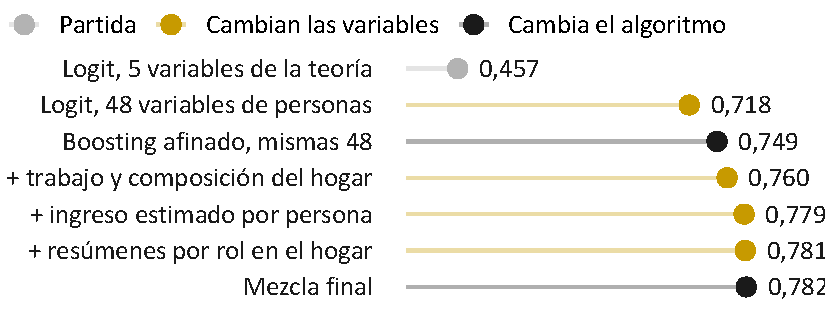
\includegraphics[width=\linewidth]{escalera_completa}
    \column{0.32\textwidth}
      \footnotesize
      \textbf{Suma de los saltos}
      \begin{itemize}
        \item \textcolor{andesaccent}{\textbf{Variables}}: $+0{,}292$.
        \item \textbf{Algoritmo}: $+0{,}032$.
      \end{itemize}
      La variable que más aportó predice el ingreso de cada persona con un modelo
      auxiliar y lo suma al hogar.
  \end{columns}
  \takeaway{La mejor inversión fue entender el hogar, no elegir el algoritmo.}
  \fuente{F1 en holdout. Fuente: views/tablas/leaderboard\_interno.csv y nivel7/ (ablacion\_etapa1, resumen\_etapa2, etapa6\_ablacion, etapa7\_a, etapa18\_resumen).}
  \note{
    \textbf{Qué decir.} Poniendo la comparación en perspectiva: toda la diferencia entre
    algoritmos que acabamos de ver suma 0,03 de F1. Construir variables desde las
    personas, y sobre todo predecir el ingreso de cada persona, sumó 0,29.\\[3pt]
    \textbf{Pregunta difícil: ¿no depende del orden de los pasos?} Sí, la descomposición
    es secuencial. Pero en cualquier orden el contraste es grande: con LightGBM fijo las
    variables nuevas suman 0,032, más que toda la diferencia entre Logit y boosting.
  }
\end{frame}

\begin{frame}{Con las variables de ingreso, todos los algoritmos convergen}
  \begin{columns}[c]
    \column{0.55\textwidth}
      \centering\scriptsize\renewcommand{\arraystretch}{1.1}
      \begin{tabular}{@{}lcc@{}}
        \toprule
        Base de 1.324 variables & F1 holdout & Corr.\ OOF \\
        \midrule
        \textbf{LightGBM} & \textbf{0,781} & 1 \\
        CatBoost & 0,779 & 0,994 \\
        AutoGluon (AutoML) & 0,777 & 0,990 \\
        RealMLP (red neuronal) & 0,775 & 0,984 \\
        TabM (red neuronal) & 0,767 & 0,977 \\
        \bottomrule
      \end{tabular}
    \column{0.43\textwidth}
      \footnotesize
      \textbf{Intuición.} Si todos predicen casi lo mismo, la información se agotó en las
      variables.
      \begin{itemize}
        \item Corr.\ OOF: correlación de sus predicciones fuera de fold con las de LightGBM; entre 0,98 y 0,99.
        \item AutoGluon sobre la base cruda, sin nuestras variables: 0,763.
        \item Mezclar los mejores suma una milésima (0,782).
      \end{itemize}
  \end{columns}
  \takeaway{El techo es común a todos: es de información, no de algoritmo.}
  \fuente{Fuente: views/tablas/nivel7/etapa7\_b.csv, etapa10\_candidatos.csv, etapa12\_resumen.csv, etapa18\_resumen.csv.}
  \note{
    \textbf{Qué decir.} Fuera de la lista del curso probamos CatBoost, redes neuronales
    tabulares y AutoML. Con nuestras variables todos quedan a menos de 0,015 de LightGBM y
    sus predicciones son casi idénticas. AutoGluon con la base cruda pierde 1,7 puntos: lo
    que le falta son nuestras variables, no capacidad de modelar.\\[3pt]
    \textbf{Pregunta difícil: ¿por qué gana LightGBM y no la red?} Con datos tabulares de
    este tamaño, los árboles con boosting suelen ganar a las redes; aquí la diferencia es de
    0,005, del orden del efecto mínimo detectable.
  }
\end{frame}

%% ============================================================
\section{Conclusión}
%% ============================================================
\begin{frame}{Más complejidad compra 6 puntos de F1 y protege más a los más pobres}
  \centering\footnotesize\renewcommand{\arraystretch}{1.12}
  \begin{tabular}{@{}lccc@{}}
    \toprule
    & Encuesta corta (Logit) & Logit completo & Mejor modelo \\
    \midrule
    Variables & 8 & 48 & 1.324 + auxiliares \\
    F1 holdout & 0,664 & 0,718 & 0,782 \\
    Subcobertura & 26,0\,\% & 23,2\,\% & 18,2\,\% \\
    Filtración & 39,8\,\% & 32,7\,\% & 25,1\,\% \\
    Excluidos en pobreza extrema & 16,1\,\% & 14,8\,\% & 11,2\,\% \\
    Interpretación & coeficientes & coeficientes & importancia y curvas \\
    Costo de recolección & bajo & medio & alto (módulo laboral) \\
    \bottomrule
  \end{tabular}
  \vspace{0.2cm}

  \raggedright\footnotesize
  Pobreza extrema: ingreso menor a la mitad de la línea, como porcentaje de los pobres excluidos.
  \takeaway{La complejidad se justifica por a quién deja de excluir, no por el F1 en sí.}
  \fuente{Holdout, umbral elegido con OOF. Fuente: views/tablas/nivel7/etapa15\_pesos\_bienestar.csv (mejor modelo: mezcla sin el modelo limpio).}
  \note{
    \textbf{Qué decir.} El trade-off concreto: pasar de 8 preguntas a un Logit completo y
    luego al mejor modelo baja la subcobertura de 26 a 18\,\% y la filtración de 40 a
    25\,\%. Y no solo excluye menos: los que excluye están más cerca de la línea.\\[3pt]
    \textbf{Pregunta difícil: ¿el mejor modelo es interpretable?} No como un Logit, pero
    sus decisiones se explican con dos cosas: ingreso predicho y vivienda. Un EBM llega a
    0,777 con curvas legibles, por si la agencia exige transparencia.
  }
\end{frame}

\begin{frame}{¿El modelo con más score en Kaggle? No necesariamente}
  \small
  \textbf{Lo que recomendaríamos a una agencia}
  \begin{enumerate}
    \item \textbf{Elegir por el costo de los errores, no por F1:} el F1 supone que excluir y
      filtrar cuestan igual; una agencia puede preferir más cobertura.
    \item \textbf{LightGBM solo, no la mezcla:} rinde igual (diferencia de milésimas) y es más
      simple de mantener y auditar.
    \item \textbf{Si exige transparencia:} un EBM (0,777) o un Logit (0,718) con el mismo
      módulo laboral, aceptando más subcobertura.
    \item \textbf{Si solo hay encuesta corta:} el Logit de 8 preguntas como filtro, con un
      umbral más bajo y verificación posterior.
  \end{enumerate}
  \takeaway{La mejor decisión depende de qué se puede medir y de cuánto cuesta excluir a un pobre.}
  \fuente{Fuente: views/tablas/nivel7/etapa15\_resumen.csv (EBM); views/tablas/leaderboard\_interno.csv; views/tablas/nivel7/etapa18\_resumen.csv.}
  \note{
    \textbf{Qué decir.} No necesariamente el de mayor Kaggle. La diferencia entre la
    mezcla y LightGBM solo es de milésimas, así que recomendamos el más simple. Si la
    agencia necesita explicar cada decisión, un EBM pierde medio punto. Y si solo puede
    pagar una encuesta corta, debe compensar con un umbral más bajo y verificación.\\[3pt]
    \textbf{Pregunta difícil: ¿por qué no recomiendan directamente el Logit, que es
    transparente?} Porque excluye a 5 puntos más de pobres y más de ellos en pobreza
    extrema; esa es una pérdida de bienestar que hay que poner en la balanza.
  }
\end{frame}

%% ============================================================
%% Apéndice
%% ============================================================
\appendix
\diapositivaglosario

\begin{frame}{Apéndice: hiperparámetros del LightGBM ganador}
  \centering\footnotesize\renewcommand{\arraystretch}{1.12}
  \begin{tabular}{@{}llll@{}}
    \toprule
    Hiperparámetro & Rango explorado & Elegido & Lectura \\
    \midrule
    Número de árboles & [200, 2000] & 1.852 & muchos árboles \\
    Tasa de aprendizaje & $10^{[-3,\,-0{,}7]}$ & 0,011 & pasos pequeños \\
    Profundidad máxima & [3, 12] & 12 (31 hojas) & árboles medianos \\
    Mínimo de hogares por hoja & [10, 200] & 171 & no memoriza casos \\
    Variables por corte & [0,2; 1] & 0,82 & algo de azar \\
    Hogares por árbol & [0,5; 1] & 0,70 & algo de azar \\
    Ganancia mínima para cortar & $10^{[-10,\,1]}$ & $7\times10^{-10}$ & sin restricción \\
    \bottomrule
  \end{tabular}
  \fuente{Hipercubo latino de 50 configuraciones, validación cruzada de 5 folds sobre las 48 variables. Fuente: views/tablas/leaderboard\_interno.csv (n6\_lightgbm).}
  \note{Respaldo: la configuración que se reutilizó en todo el nivel 7.}
\end{frame}

\begin{frame}{Apéndice: en CV repetida ninguna alternativa mejora de forma detectable}
  \centering\scriptsize
  \begin{tabular}{@{}lccc@{}}
    \toprule
    Candidato & F1 CV repetida (EE) & $\Delta$ vs.\ LightGBM [IC 95\,\%] & F1 holdout [IC 95\,\%] \\
    \midrule
    LightGBM base & 0,7752 (0,0008) & & 0,7806 [0,7731; 0,7885] \\
    + redes (mezcla sin limpio) & 0,7758 (0,0008) & $+0{,}0006$ [$-0{,}0001$; $+0{,}0013$] & 0,7820 [0,7743; 0,7897] \\
    \textbf{+ redes + limpio (final)} & \textbf{0,7759 (0,0008)} & $+0{,}0007$ [$+0{,}0002$; $+0{,}0012$] & 0,7817 [0,7742; 0,7894] \\
    CatBoost & 0,7722 (0,0007) & $-0{,}0030$ [$-0{,}0042$; $-0{,}0018$] & 0,7786 [0,7707; 0,7864] \\
    Rediseño desde cero & 0,7478 (0,0008) & $-0{,}0274$ [$-0{,}0289$; $-0{,}0260$] & 0,7499 [0,7420; 0,7581] \\
    \bottomrule
  \end{tabular}
  \fuente{IC pareados ingenuos (15 pares). Con la corrección de Nadeau y Bengio el IC del modelo final es [$-0{,}0004$; $+0{,}0017$]. Fuente: views/tablas/nivel7/etapa16\_fase1\_resumen.csv, etapa18\_resumen.csv.}
  \note{Respaldo: CatBoost pierde con un IC que excluye cero; la mezcla gana por milésimas.}
\end{frame}

\end{document}
"
%% ============================================================
\documentclass[aspectratio=169,11pt]{beamer}
%% Preamble: packages and theme. Keep design changes in beamerthemeUniandes.sty
\usepackage[utf8]{inputenc}
\usepackage[T1]{fontenc}
\usepackage[spanish,es-nodecimaldot,es-noshorthands]{babel}
\usepackage{amsmath,amssymb}
\usepackage{graphicx}
\usepackage{booktabs}
\usepackage[round]{natbib}
\usetheme{Uniandes}

%% ---- Agregados para el Problem Set 2 (no cambian el diseño) ----
% Algunas instalaciones de MiKTeX no registran el mapa de Source Sans; se carga aquí.
\pdfmapfile{+SourceSansThree.map}
\usepackage{array}
\usepackage{xspace}
\usetikzlibrary{positioning,arrows.meta,decorations.pathreplacing}
\graphicspath{{../figuras/}{../../../views/figuras/}{../../../views/figuras/nivel7/}}

% Notas del presentador: el PDF de entrega no las muestra; la versión *_notas
% se compila con \def\connotas{} antes del documento y las intercala.
\ifdefined\connotas
  \setbeameroption{show notes}
\else
  \setbeameroption{hide notes}
\fi
\setbeamerfont{note page}{size=\small}
\setbeamertemplate{note page}{%
  \vspace{0.3cm}\insertslideintonotes{0.25}\par\vspace{0.2cm}
  \begin{minipage}{0.95\textwidth}\insertnote\end{minipage}}

% F1 público de Kaggle del mejor modelo (n18), tal como lo muestra la Overview.
\def\kagglepublico{0,78}

% Tabla pequeña con letra reducida
\newcommand{\tablachica}{\footnotesize\renewcommand{\arraystretch}{1.12}}
% Fuente de una figura o tabla, al pie
\newcommand{\fuente}[1]{\par\vspace{2pt}{\tiny\color{andesgray}#1\par}}
% Títulos sin cortar palabras con guion: se hace dentro de la plantilla del título
% (beamerthemeUniandes.sty), porque el minipage del título reinicia la alineación.
% Cajas de los diagramas sin guiones
\tikzset{every node/.append style={execute at begin node={\hyphenpenalty=10000\exhyphenpenalty=10000}}}

%% ============================================================
%%  Piezas comunes a los dos decks: Best Model Overview y glosario
%% ============================================================

% ---- Best Model Overview (diapositiva obligatoria, primera de cada deck) ----
\newcommand{\diapositivaoverview}{%
\begin{frame}{Best Model Overview}
  {Ingreso predicho por persona + LightGBM \;|\; Equipo 06, MECA 4107}
  \vspace{-0.1cm}
  \begin{columns}[T]
    \column{0.37\textwidth}\centering \keyfig{\kagglepublico}{F1 público en Kaggle}
    \column{0.30\textwidth}\centering \keyfig{0,782}{F1 en holdout, IC 95\,\% [0,774; 0,789]}
    \column{0.30\textwidth}\centering \keyfig{0,776}{F1 en CV repetida (15 evaluaciones)}
  \end{columns}
  \vspace{0.15cm}
  \footnotesize
  \begin{columns}[T]
    \column{0.49\textwidth}
      \textbf{Especificación}
      \begin{itemize}
        \item \textbf{Variable clave:} el ingreso de cada persona, predicho con lo que el test
          sí trae y sumado al hogar (1.324 variables en total).
        \item \textbf{Algoritmo:} LightGBM (76\,\%) mezclado con dos redes (19\,\%) y un
          rediseño desde cero (5\,\%); pesos elegidos fuera de muestra.
        \item \textbf{Regla:} pobre si $P(\text{pobre}) \geq 0{,}36$.
      \end{itemize}
    \column{0.49\textwidth}
      \textbf{Mensajes}
      \begin{enumerate}
        \item Las variables aportaron \textbf{9 veces más} F1 que los algoritmos.
        \item El techo (${\approx}\,0{,}78$) viene sobre todo de la información que falta.
        \item Excluye al 18\,\% de los pobres, casi todos cerca de la línea.
      \end{enumerate}
  \end{columns}
  \fuente{F1: media armónica de precisión y recall de la clase pobre. Holdout: 20\,\% del train nunca usado para decidir. Fuente: views/tablas/nivel7/etapa18\_resumen.csv.}
  \note{
    \textbf{Qué decir (1 min).} Nuestro mejor modelo clasifica hogares pobres con F1 de
    0,782 en datos que nunca usamos para decidir. La pieza clave no es el algoritmo sino
    una variable: predecimos cuánto gana cada persona con lo que el test sí trae
    (ocupación, horas, cotización) y lo sumamos al hogar. Tres mensajes: las variables
    pesan 9 veces más que el algoritmo, hay un techo que viene de los datos y los errores
    se concentran cerca de la línea.\\[3pt]
    \textbf{Pregunta difícil: ¿por qué una mezcla y no un solo modelo?} La mezcla gana
    +0,0007 en CV repetida frente a LightGBM solo. El IC ingenuo [+0,0002; +0,0012] excluye
    cero; el corregido por dependencia entre folds no. Es una mejora marginal: en la
    práctica LightGBM solo rinde igual.
  }
\end{frame}}

% ---- Glosario (apéndice de ambos decks, dos diapositivas) ----
\newcommand{\filaglosario}[2]{\textbf{#1} & #2 \\}
\newcommand{\diapositivaglosario}{%
\begin{frame}{Glosario (1/2): métricas y errores}
  \footnotesize\renewcommand{\arraystretch}{1.25}
  \begin{tabular}{@{}p{0.2\textwidth}p{0.76\textwidth}@{}}
    \toprule
    \filaglosario{Precisión}{De los hogares que el programa atiende, qué parte es pobre. $1-$precisión $=$ \textbf{filtración}: no pobres que reciben el beneficio.}
    \filaglosario{Recall}{De los hogares pobres, qué parte atiende el programa. $1-$recall $=$ \textbf{subcobertura}: pobres excluidos.}
    \filaglosario{F1}{Media armónica de precisión y recall: solo es alta si ambas lo son. No premia a los no pobres bien clasificados.}
    \filaglosario{Umbral}{Probabilidad a partir de la cual un hogar se clasifica como pobre. Bajarlo cubre más pobres a cambio de más filtración.}
    \filaglosario{IC 95\,\%}{Rango de valores compatibles con los datos. Si el IC de una diferencia incluye cero, no podemos afirmar que haya mejora.}
    \filaglosario{Efecto mínimo detectable}{La mejora más pequeña que el diseño detectaría con probabilidad 0,8.}
    \bottomrule
  \end{tabular}
  \note{Glosario de apoyo; se muestra solo si lo preguntan.}
\end{frame}
\begin{frame}{Glosario (2/2): validación y variables}
  \footnotesize\renewcommand{\arraystretch}{1.25}
  \begin{tabular}{@{}p{0.2\textwidth}p{0.76\textwidth}@{}}
    \toprule
    \filaglosario{Holdout}{20\,\% del train (32.993 hogares) apartado al inicio; solo se usa para medir, nunca para decidir.}
    \filaglosario{Validación cruzada}{El 80\,\% restante se parte en 5 bloques (folds): se entrena con 4 y se evalúa en el quinto, rotando.}
    \filaglosario{Fuera de fold (OOF)}{La predicción de cada hogar hecha por un modelo que no lo vio. Con ella se eligen umbral, pesos e hiperparámetros.}
    \filaglosario{CV repetida}{La validación cruzada repetida con 3 particiones nuevas: 15 evaluaciones para medir la variabilidad.}
    \filaglosario{Auxiliar de ingreso}{Modelo que predice el ingreso de cada persona con variables que el test sí trae; sumado al hogar, entra como variable.}
    \filaglosario{OOF anidada}{El auxiliar que alimenta a un hogar no vio ese hogar ni su fold de validación: así no se filtra la respuesta.}
    \bottomrule
  \end{tabular}
  \note{Glosario de apoyo; se muestra solo si lo preguntan.}
\end{frame}}


\title[Predicting Poverty: Algorithm Comparison]{Predicting Poverty: Algorithm Comparison}
\author[Labastidas y Garcia | Equipo 06]{Esteban David Labastidas Martínez \and Neislen Stiven Garcia Silva}
\institute{Facultad de Economía\\ Universidad de los Andes}
\date[Oct 2026]{Bogotá, octubre de 2026}

\begin{document}
\andessectionslidesfalse

%% 1. Best Model Overview (obligatoria)
\diapositivaoverview

%% ============================================================
\section{Datos}
%% ============================================================
\begin{frame}{La pobreza responde a umbrales e interacciones: terreno favorable para los árboles}
  \begin{columns}[c]
    \column{0.60\textwidth}
      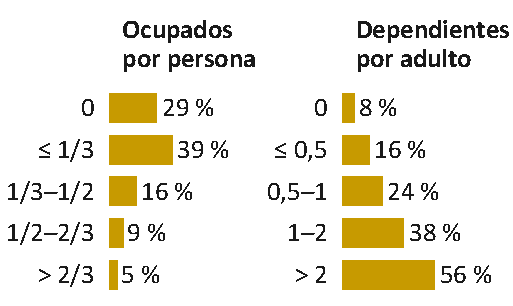
\includegraphics[width=\linewidth]{correlatos_pobreza}
    \column{0.38\textwidth}
      \footnotesize
      \textbf{Intuición.} Un modelo lineal suma efectos; un árbol corta en umbrales y
      combina variables.
      \begin{itemize}
        \item \textbf{No linealidad:} con más ocupados la pobreza sube de 29\,\% a 39\,\% y
          luego cae a 5\,\%.
        \item \textbf{Interacción:} el arriendo pesa distinto si la vivienda es propia o
          arrendada (la interacción más fuerte en un EBM).
        \item \textbf{Desbalance:} 20\,\% de pobres; el umbral se elige fuera de fold.
      \end{itemize}
  \end{columns}
  \takeaway{Esperamos que los métodos de árboles con muchas variables ganen a los lineales.}
  \fuente{Fuente: base de hogares de train (scripts/13\_figuras\_presentacion.R); views/tablas/nivel7/etapa15\_ebm\_importancia.csv.}
  \note{
    \textbf{Qué decir.} Antes de comparar, una predicción desde los datos. La pobreza no
    responde de forma lineal: con cero ocupados es menor que con un tercio, porque hay
    pensionados. Y las variables interactúan: pagar arriendo no significa lo mismo en una
    casa propia que en una arrendada. Eso favorece a los árboles, que cortan en umbrales y
    combinan variables sin que se las especifiquemos.\\[3pt]
    \textbf{Pregunta difícil: ¿no basta con interacciones en el Logit?} Se podrían
    agregar, pero habría que elegirlas a mano entre más de mil pares posibles; los árboles
    las buscan solos. El costo es la interpretabilidad.
  }
\end{frame}

%% ============================================================
\section{Comparación de algoritmos}
%% ============================================================
\begin{frame}{Cancha nivelada: mismas 48 variables, misma receta y misma validación}
  \centering\scriptsize\renewcommand{\arraystretch}{1.12}
  \begin{tabular}{@{}lllr@{}}
    \toprule
    Algoritmo & Búsqueda (validación cruzada de 5 folds) & Elegido & Configs. \\
    \midrule
    LPM y Logit & sin hiperparámetros & & 1 \\
    Elastic Net & grilla: penalización $10^{[-5,\,0]}$ $\times$ mezcla L1/L2 [0, 1] & 0,0002; 0,2 & 120 \\
    CART & grilla: complejidad $10^{[-5,\,-1]}$ $\times$ profundidad [3, 15] & $6\times10^{-5}$; 10 & 36 \\
    Naive Bayes & grilla: suavizado [0,5; 1,5] $\times$ Laplace [0, 3] & 0,5; 0 & 16 \\
    Random Forest & hipercubo: variables por corte [3, 25] $\times$ tamaño de hoja [5, 60] & 23; 24 & 15 \\
    XGBoost & hipercubo: árboles [200, 1000] $\times$ profundidad [3, 8] $\times$ tasa $10^{[-3,\,-1]}$ & 781; 6; 0,020 & 20 \\
    LightGBM & hipercubo de 7 hiperparámetros & ver apéndice & 50 \\
    \bottomrule
  \end{tabular}
  \vspace{0.25cm}

  \raggedright\small
  Todos usan la misma receta (imputación, dummies y escalado ajustados dentro de cada
  fold), el umbral elegido con predicciones fuera de fold y el mismo holdout del 20\,\%.
  \takeaway{Las diferencias de F1 reflejan el algoritmo, no los datos que recibe.}
  \fuente{Fuente: views/tablas/leaderboard\_interno.csv (columnas busqueda e hiperparametros).}
  \note{
    \textbf{Qué decir.} Para que la comparación sea justa, todos los algoritmos reciben
    las mismas 48 variables, el mismo preprocesamiento ajustado solo con los datos de
    entrenamiento de cada fold, y eligen hiperparámetros con validación cruzada de 5 folds.
    Grilla regular cuando hay 1 o 2 hiperparámetros, hipercubo latino cuando hay más.\\[3pt]
    \textbf{Pregunta difícil: ¿no tienen ventaja los que recibieron más configuraciones?}
    LightGBM probó 50 y XGBoost 20, pero XGBoost ya llegaba a 0,746 frente a 0,749: la
    ventaja de tuning es de 0,003. Elastic Net probó 120 y empata con el Logit sin tuning.
  }
\end{frame}

\begin{frame}{Con las mismas variables, el boosting gana y Naive Bayes queda 11 puntos atrás}
  \begin{columns}[c]
    \column{0.60\textwidth}
      \centering\scriptsize\renewcommand{\arraystretch}{1.1}
      \begin{tabular}{@{}lcccc@{}}
        \toprule
        Algoritmo & F1 CV & F1 holdout & Filtración & Subcob. \\
        \midrule
        \textbf{Boosting (LightGBM)} & \textbf{0,744} & \textbf{0,749} & 29,3\,\% & 20,4\,\% \\
        Boosting (XGBoost) & 0,740 & 0,746 & 29,6\,\% & 20,6\,\% \\
        Random Forest & 0,726 & 0,734 & 32,0\,\% & 20,2\,\% \\
        Elastic Net & 0,717 & 0,718 & 33,2\,\% & 22,4\,\% \\
        Logit & 0,717 & 0,718 & 32,7\,\% & 23,2\,\% \\
        CART & 0,697 & 0,701 & 34,3\,\% & 24,8\,\% \\
        LPM & 0,690 & 0,691 & 34,9\,\% & 26,3\,\% \\
        Naive Bayes & 0,643 & 0,640 & 44,0\,\% & 25,2\,\% \\
        \bottomrule
      \end{tabular}
    \column{0.38\textwidth}
      \footnotesize
      \textbf{Filtración} $=$ no pobres entre los atendidos ($1-$precisión).
      \textbf{Subcobertura} $=$ pobres excluidos ($1-$recall).
      \begin{itemize}
        \item El orden se repite en CV y en holdout: no es ruido de una partición.
        \item Los mejores ganan sobre todo en filtración.
        \item Naive Bayes supone variables independientes; aquí están muy correlacionadas.
      \end{itemize}
  \end{columns}
  \takeaway{Los dos más cercanos al ganador son Random Forest y Elastic Net (con Logit).}
  \fuente{Holdout de 32.993 hogares; umbral elegido con OOF. Fuente: views/tablas/comparacion\_algoritmos.csv; views/tablas/leaderboard\_interno.csv.}
  \note{
    \textbf{Qué decir.} Esta es la comparación de los siete algoritmos del curso con las
    mismas variables. El boosting queda primero y Naive Bayes último. El orden es el mismo
    en validación cruzada y en holdout. Los dos contendores más cercanos son Random Forest
    y Elastic Net, que empata con el Logit.\\[3pt]
    \textbf{Pregunta difícil: ¿son significativas estas diferencias?} Con 32.993 hogares,
    el efecto mínimo detectable en holdout está entre 0,0025 y 0,006 según el par: las
    brechas de 0,015 o más están claramente por encima; la de XGBoost frente a LightGBM, no.
  }
\end{frame}

\begin{frame}{Random Forest cubre igual que el boosting, pero filtra más}
  \begin{columns}[T]
    \column{0.50\textwidth}
      \centering\footnotesize
      \begin{tabular}{@{}lcc@{}}
        \toprule
        Holdout, 48 variables & Random Forest & XGBoost \\
        \midrule
        Recall (cobertura) & 0,798 & 0,794 \\
        Precisión & 0,680 & 0,704 \\
        No pobres incluidos & 2.483 & 2.206 \\
        Pobres excluidos & 1.332 & 1.358 \\
        F1 & 0,734 & 0,746 \\
        \bottomrule
      \end{tabular}
      \vspace{0.25cm}

      \begin{tabular}{@{}lcc@{}}
        \toprule
        Con variables de ingreso & F1 holdout & Brecha \\
        \midrule
        LightGBM (todas) & 0,781 & \\
        Random Forest (60 mejores) & 0,776 & $-0{,}005$ \\
        \bottomrule
      \end{tabular}
    \column{0.46\textwidth}
      \footnotesize
      \textbf{Intuición.} Random Forest promedia árboles profundos que aprenden lo mismo en
      paralelo; el boosting suma árboles pequeños que corrigen los errores de los
      anteriores, como los hogares cerca de la línea.
      \begin{itemize}
        \item Misma cobertura, pero 277 no pobres más incluidos: la brecha está en la
          precisión.
        \item Con las variables de ingreso la brecha baja de 0,012 a 0,005: con mejores
          variables, el algoritmo importa menos.
      \end{itemize}
  \end{columns}
  \takeaway{La ventaja del boosting está en la precisión: incluye menos no pobres.}
  \fuente{Fuente: views/tablas/leaderboard\_interno.csv; views/tablas/nivel7/etapa9\_candidatos.csv (Random Forest con las 60 variables de un algoritmo genético; no es cancha nivelada).}
  \note{
    \textbf{Qué decir.} Random Forest es el contendor más cercano. Cubre a los mismos
    pobres que el boosting, pero incluye 277 no pobres más. Una lectura: el bosque promedia
    árboles independientes, mientras el boosting agrega árboles enfocados en los errores
    que quedan, que están cerca de la línea. Con las variables de ingreso, la brecha se
    reduce a la mitad.\\[3pt]
    \textbf{Pregunta difícil: ¿la comparación del nivel 7 es justa?} No del todo: el bosque
    usó 60 variables y LightGBM todas. Por eso solo la usamos para mostrar que la brecha
    se achica, no para medirla.
  }
\end{frame}

\begin{frame}{Elastic Net empata con el Logit: la brecha con el boosting es por la linealidad}
  \begin{columns}[T]
    \column{0.48\textwidth}
      \footnotesize
      \textbf{Intuición.} Elastic Net penaliza coeficientes para evitar el sobreajuste. Con
      131.967 hogares y 48 variables no hay sobreajuste que evitar.
      \begin{itemize}
        \item La validación cruzada elige una penalización casi nula (0,0002).
        \item Mismo F1 en holdout que el Logit: 0,718.
        \item LPM (probabilidad lineal): 0,691, es decir 0,027 menos que el Logit.
      \end{itemize}
    \column{0.48\textwidth}
      \footnotesize
      \textbf{Lo que cuesta la linealidad frente al boosting}
      \begin{itemize}
        \item F1: 0,718 frente a 0,749 ($-0{,}031$).
        \item Subcobertura 22,4\,\% frente a 20,4\,\%: unos 130 pobres más excluidos en
          el holdout.
        \item A cambio, cada coeficiente se puede leer y auditar.
      \end{itemize}
  \end{columns}
  \takeaway{Regularizar no ayuda con muchos datos; lo que falta son umbrales e interacciones.}
  \fuente{Fuente: views/tablas/leaderboard\_interno.csv (n4\_elastic\_net, n3\_logit, n3\_lpm, n6\_lightgbm).}
  \note{
    \textbf{Qué decir.} El segundo contendor es Elastic Net. La validación cruzada elige
    casi no penalizar, porque con más de 130 mil hogares y 48 variables no hay sobreajuste.
    Por eso empata con el Logit. Lo que lo separa del boosting no es la regularización sino
    la forma funcional: no capta umbrales ni interacciones.\\[3pt]
    \textbf{Pregunta difícil: ¿cuántos pobres más excluye?} Con 6.605 pobres en el
    holdout, 2 puntos de subcobertura son unos 130 hogares (1.478 frente a 1.347
    excluidos).
  }
\end{frame}

\begin{frame}{Balancear las clases no mejora: solo mueve el umbral}
  \begin{columns}[c]
    \column{0.50\textwidth}
      \centering\footnotesize
      \begin{tabular}{@{}lcc@{}}
        \toprule
        XGBoost, 48 variables & F1 holdout & Umbral óptimo \\
        \midrule
        Sin balancear & 0,746 & 0,36 \\
        SMOTE & 0,745 & 0,34 \\
        Pesos de clase & 0,744 & 0,66 \\
        Submuestreo & 0,747 & 0,69 \\
        \bottomrule
      \end{tabular}
    \column{0.46\textwidth}
      \footnotesize
      \textbf{Intuición.} Balancear infla la probabilidad de ser pobre. Si después se elige
      el umbral que maximiza F1, ese umbral sube y deshace el cambio.
      \begin{itemize}
        \item Diferencias de F1 de 0,002 o menos, dentro del ruido.
        \item El umbral pasa de 0,36 a 0,66--0,69 con pesos o submuestreo.
      \end{itemize}
  \end{columns}
  \takeaway{Con el umbral elegido fuera de fold, el desbalance ya está resuelto.}
  \fuente{Fuente: views/tablas/leaderboard\_interno.csv (n4\_xgboost y n5\_*).}
  \note{
    \textbf{Qué decir.} Probamos las tres estrategias clásicas sobre el mejor algoritmo
    de ese nivel. Ninguna cambia el F1 más allá de 0,002. Lo que sí cambia es el umbral
    óptimo, porque el balanceo solo reescala las probabilidades.\\[3pt]
    \textbf{Pregunta difícil: ¿y si no se eligiera el umbral?} Con el umbral fijo en 0,5,
    esperaríamos que balancear sí ayudara, porque acerca las probabilidades al punto de
    corte (no lo medimos). Elegir el umbral es la forma directa de lograr lo mismo.
  }
\end{frame}

\begin{frame}{Cambiar las variables vale 9 veces más que cambiar el algoritmo}
  \begin{columns}[c]
    \column{0.66\textwidth}
      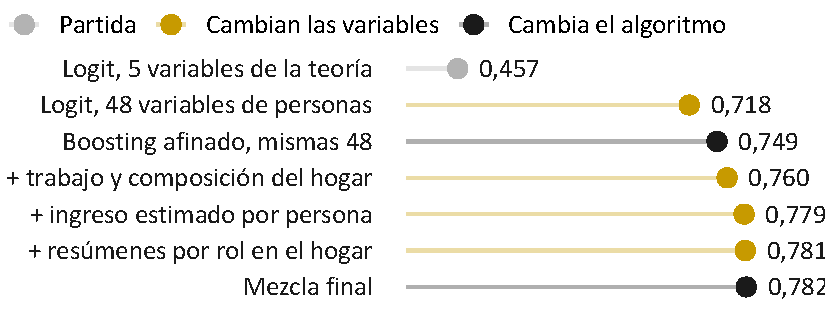
\includegraphics[width=\linewidth]{escalera_completa}
    \column{0.32\textwidth}
      \footnotesize
      \textbf{Suma de los saltos}
      \begin{itemize}
        \item \textcolor{andesaccent}{\textbf{Variables}}: $+0{,}292$.
        \item \textbf{Algoritmo}: $+0{,}032$.
      \end{itemize}
      La variable que más aportó predice el ingreso de cada persona con un modelo
      auxiliar y lo suma al hogar.
  \end{columns}
  \takeaway{La mejor inversión fue entender el hogar, no elegir el algoritmo.}
  \fuente{F1 en holdout. Fuente: views/tablas/leaderboard\_interno.csv y nivel7/ (ablacion\_etapa1, resumen\_etapa2, etapa6\_ablacion, etapa7\_a, etapa18\_resumen).}
  \note{
    \textbf{Qué decir.} Poniendo la comparación en perspectiva: toda la diferencia entre
    algoritmos que acabamos de ver suma 0,03 de F1. Construir variables desde las
    personas, y sobre todo predecir el ingreso de cada persona, sumó 0,29.\\[3pt]
    \textbf{Pregunta difícil: ¿no depende del orden de los pasos?} Sí, la descomposición
    es secuencial. Pero en cualquier orden el contraste es grande: con LightGBM fijo las
    variables nuevas suman 0,032, más que toda la diferencia entre Logit y boosting.
  }
\end{frame}

\begin{frame}{Con las variables de ingreso, todos los algoritmos convergen}
  \begin{columns}[c]
    \column{0.55\textwidth}
      \centering\scriptsize\renewcommand{\arraystretch}{1.1}
      \begin{tabular}{@{}lcc@{}}
        \toprule
        Base de 1.324 variables & F1 holdout & Corr.\ OOF \\
        \midrule
        \textbf{LightGBM} & \textbf{0,781} & 1 \\
        CatBoost & 0,779 & 0,994 \\
        AutoGluon (AutoML) & 0,777 & 0,990 \\
        RealMLP (red neuronal) & 0,775 & 0,984 \\
        TabM (red neuronal) & 0,767 & 0,977 \\
        \bottomrule
      \end{tabular}
    \column{0.43\textwidth}
      \footnotesize
      \textbf{Intuición.} Si todos predicen casi lo mismo, la información se agotó en las
      variables.
      \begin{itemize}
        \item Corr.\ OOF: correlación de sus predicciones fuera de fold con las de LightGBM; entre 0,98 y 0,99.
        \item AutoGluon sobre la base cruda, sin nuestras variables: 0,763.
        \item Mezclar los mejores suma una milésima (0,782).
      \end{itemize}
  \end{columns}
  \takeaway{El techo es común a todos: es de información, no de algoritmo.}
  \fuente{Fuente: views/tablas/nivel7/etapa7\_b.csv, etapa10\_candidatos.csv, etapa12\_resumen.csv, etapa18\_resumen.csv.}
  \note{
    \textbf{Qué decir.} Fuera de la lista del curso probamos CatBoost, redes neuronales
    tabulares y AutoML. Con nuestras variables todos quedan a menos de 0,015 de LightGBM y
    sus predicciones son casi idénticas. AutoGluon con la base cruda pierde 1,7 puntos: lo
    que le falta son nuestras variables, no capacidad de modelar.\\[3pt]
    \textbf{Pregunta difícil: ¿por qué gana LightGBM y no la red?} Con datos tabulares de
    este tamaño, los árboles con boosting suelen ganar a las redes; aquí la diferencia es de
    0,005, del orden del efecto mínimo detectable.
  }
\end{frame}

%% ============================================================
\section{Conclusión}
%% ============================================================
\begin{frame}{Más complejidad compra 6 puntos de F1 y protege más a los más pobres}
  \centering\footnotesize\renewcommand{\arraystretch}{1.12}
  \begin{tabular}{@{}lccc@{}}
    \toprule
    & Encuesta corta (Logit) & Logit completo & Mejor modelo \\
    \midrule
    Variables & 8 & 48 & 1.324 + auxiliares \\
    F1 holdout & 0,664 & 0,718 & 0,782 \\
    Subcobertura & 26,0\,\% & 23,2\,\% & 18,2\,\% \\
    Filtración & 39,8\,\% & 32,7\,\% & 25,1\,\% \\
    Excluidos en pobreza extrema & 16,1\,\% & 14,8\,\% & 11,2\,\% \\
    Interpretación & coeficientes & coeficientes & importancia y curvas \\
    Costo de recolección & bajo & medio & alto (módulo laboral) \\
    \bottomrule
  \end{tabular}
  \vspace{0.2cm}

  \raggedright\footnotesize
  Pobreza extrema: ingreso menor a la mitad de la línea, como porcentaje de los pobres excluidos.
  \takeaway{La complejidad se justifica por a quién deja de excluir, no por el F1 en sí.}
  \fuente{Holdout, umbral elegido con OOF. Fuente: views/tablas/nivel7/etapa15\_pesos\_bienestar.csv (mejor modelo: mezcla sin el modelo limpio).}
  \note{
    \textbf{Qué decir.} El trade-off concreto: pasar de 8 preguntas a un Logit completo y
    luego al mejor modelo baja la subcobertura de 26 a 18\,\% y la filtración de 40 a
    25\,\%. Y no solo excluye menos: los que excluye están más cerca de la línea.\\[3pt]
    \textbf{Pregunta difícil: ¿el mejor modelo es interpretable?} No como un Logit, pero
    sus decisiones se explican con dos cosas: ingreso predicho y vivienda. Un EBM llega a
    0,777 con curvas legibles, por si la agencia exige transparencia.
  }
\end{frame}

\begin{frame}{¿El modelo con más score en Kaggle? No necesariamente}
  \small
  \textbf{Lo que recomendaríamos a una agencia}
  \begin{enumerate}
    \item \textbf{Elegir por el costo de los errores, no por F1:} el F1 supone que excluir y
      filtrar cuestan igual; una agencia puede preferir más cobertura.
    \item \textbf{LightGBM solo, no la mezcla:} rinde igual (diferencia de milésimas) y es más
      simple de mantener y auditar.
    \item \textbf{Si exige transparencia:} un EBM (0,777) o un Logit (0,718) con el mismo
      módulo laboral, aceptando más subcobertura.
    \item \textbf{Si solo hay encuesta corta:} el Logit de 8 preguntas como filtro, con un
      umbral más bajo y verificación posterior.
  \end{enumerate}
  \takeaway{La mejor decisión depende de qué se puede medir y de cuánto cuesta excluir a un pobre.}
  \fuente{Fuente: views/tablas/nivel7/etapa15\_resumen.csv (EBM); views/tablas/leaderboard\_interno.csv; views/tablas/nivel7/etapa18\_resumen.csv.}
  \note{
    \textbf{Qué decir.} No necesariamente el de mayor Kaggle. La diferencia entre la
    mezcla y LightGBM solo es de milésimas, así que recomendamos el más simple. Si la
    agencia necesita explicar cada decisión, un EBM pierde medio punto. Y si solo puede
    pagar una encuesta corta, debe compensar con un umbral más bajo y verificación.\\[3pt]
    \textbf{Pregunta difícil: ¿por qué no recomiendan directamente el Logit, que es
    transparente?} Porque excluye a 5 puntos más de pobres y más de ellos en pobreza
    extrema; esa es una pérdida de bienestar que hay que poner en la balanza.
  }
\end{frame}

%% ============================================================
%% Apéndice
%% ============================================================
\appendix
\diapositivaglosario

\begin{frame}{Apéndice: hiperparámetros del LightGBM ganador}
  \centering\footnotesize\renewcommand{\arraystretch}{1.12}
  \begin{tabular}{@{}llll@{}}
    \toprule
    Hiperparámetro & Rango explorado & Elegido & Lectura \\
    \midrule
    Número de árboles & [200, 2000] & 1.852 & muchos árboles \\
    Tasa de aprendizaje & $10^{[-3,\,-0{,}7]}$ & 0,011 & pasos pequeños \\
    Profundidad máxima & [3, 12] & 12 (31 hojas) & árboles medianos \\
    Mínimo de hogares por hoja & [10, 200] & 171 & no memoriza casos \\
    Variables por corte & [0,2; 1] & 0,82 & algo de azar \\
    Hogares por árbol & [0,5; 1] & 0,70 & algo de azar \\
    Ganancia mínima para cortar & $10^{[-10,\,1]}$ & $7\times10^{-10}$ & sin restricción \\
    \bottomrule
  \end{tabular}
  \fuente{Hipercubo latino de 50 configuraciones, validación cruzada de 5 folds sobre las 48 variables. Fuente: views/tablas/leaderboard\_interno.csv (n6\_lightgbm).}
  \note{Respaldo: la configuración que se reutilizó en todo el nivel 7.}
\end{frame}

\begin{frame}{Apéndice: en CV repetida ninguna alternativa mejora de forma detectable}
  \centering\scriptsize
  \begin{tabular}{@{}lccc@{}}
    \toprule
    Candidato & F1 CV repetida (EE) & $\Delta$ vs.\ LightGBM [IC 95\,\%] & F1 holdout [IC 95\,\%] \\
    \midrule
    LightGBM base & 0,7752 (0,0008) & & 0,7806 [0,7731; 0,7885] \\
    + redes (mezcla sin limpio) & 0,7758 (0,0008) & $+0{,}0006$ [$-0{,}0001$; $+0{,}0013$] & 0,7820 [0,7743; 0,7897] \\
    \textbf{+ redes + limpio (final)} & \textbf{0,7759 (0,0008)} & $+0{,}0007$ [$+0{,}0002$; $+0{,}0012$] & 0,7817 [0,7742; 0,7894] \\
    CatBoost & 0,7722 (0,0007) & $-0{,}0030$ [$-0{,}0042$; $-0{,}0018$] & 0,7786 [0,7707; 0,7864] \\
    Rediseño desde cero & 0,7478 (0,0008) & $-0{,}0274$ [$-0{,}0289$; $-0{,}0260$] & 0,7499 [0,7420; 0,7581] \\
    \bottomrule
  \end{tabular}
  \fuente{IC pareados ingenuos (15 pares). Con la corrección de Nadeau y Bengio el IC del modelo final es [$-0{,}0004$; $+0{,}0017$]. Fuente: views/tablas/nivel7/etapa16\_fase1\_resumen.csv, etapa18\_resumen.csv.}
  \note{Respaldo: CatBoost pierde con un IC que excluye cero; la mezcla gana por milésimas.}
\end{frame}

\end{document}
"
%% ============================================================
\documentclass[aspectratio=169,11pt]{beamer}
%% Preamble: packages and theme. Keep design changes in beamerthemeUniandes.sty
\usepackage[utf8]{inputenc}
\usepackage[T1]{fontenc}
\usepackage[spanish,es-nodecimaldot,es-noshorthands]{babel}
\usepackage{amsmath,amssymb}
\usepackage{graphicx}
\usepackage{booktabs}
\usepackage[round]{natbib}
\usetheme{Uniandes}

%% ---- Agregados para el Problem Set 2 (no cambian el diseño) ----
% Algunas instalaciones de MiKTeX no registran el mapa de Source Sans; se carga aquí.
\pdfmapfile{+SourceSansThree.map}
\usepackage{array}
\usepackage{xspace}
\usetikzlibrary{positioning,arrows.meta,decorations.pathreplacing}
\graphicspath{{../figuras/}{../../../views/figuras/}{../../../views/figuras/nivel7/}}

% Notas del presentador: el PDF de entrega no las muestra; la versión *_notas
% se compila con \def\connotas{} antes del documento y las intercala.
\ifdefined\connotas
  \setbeameroption{show notes}
\else
  \setbeameroption{hide notes}
\fi
\setbeamerfont{note page}{size=\small}
\setbeamertemplate{note page}{%
  \vspace{0.3cm}\insertslideintonotes{0.25}\par\vspace{0.2cm}
  \begin{minipage}{0.95\textwidth}\insertnote\end{minipage}}

% F1 público de Kaggle del mejor modelo (n18), tal como lo muestra la Overview.
\def\kagglepublico{0,78}

% Tabla pequeña con letra reducida
\newcommand{\tablachica}{\footnotesize\renewcommand{\arraystretch}{1.12}}
% Fuente de una figura o tabla, al pie
\newcommand{\fuente}[1]{\par\vspace{2pt}{\tiny\color{andesgray}#1\par}}
% Títulos sin cortar palabras con guion: se hace dentro de la plantilla del título
% (beamerthemeUniandes.sty), porque el minipage del título reinicia la alineación.
% Cajas de los diagramas sin guiones
\tikzset{every node/.append style={execute at begin node={\hyphenpenalty=10000\exhyphenpenalty=10000}}}

%% ============================================================
%%  Piezas comunes a los dos decks: Best Model Overview y glosario
%% ============================================================

% ---- Best Model Overview (diapositiva obligatoria, primera de cada deck) ----
\newcommand{\diapositivaoverview}{%
\begin{frame}{Best Model Overview}
  {Ingreso predicho por persona + LightGBM \;|\; Equipo 06, MECA 4107}
  \vspace{-0.1cm}
  \begin{columns}[T]
    \column{0.37\textwidth}\centering \keyfig{\kagglepublico}{F1 público en Kaggle}
    \column{0.30\textwidth}\centering \keyfig{0,782}{F1 en holdout, IC 95\,\% [0,774; 0,789]}
    \column{0.30\textwidth}\centering \keyfig{0,776}{F1 en CV repetida (15 evaluaciones)}
  \end{columns}
  \vspace{0.15cm}
  \footnotesize
  \begin{columns}[T]
    \column{0.49\textwidth}
      \textbf{Especificación}
      \begin{itemize}
        \item \textbf{Variable clave:} el ingreso de cada persona, predicho con lo que el test
          sí trae y sumado al hogar (1.324 variables en total).
        \item \textbf{Algoritmo:} LightGBM (76\,\%) mezclado con dos redes (19\,\%) y un
          rediseño desde cero (5\,\%); pesos elegidos fuera de muestra.
        \item \textbf{Regla:} pobre si $P(\text{pobre}) \geq 0{,}36$.
      \end{itemize}
    \column{0.49\textwidth}
      \textbf{Mensajes}
      \begin{enumerate}
        \item Las variables aportaron \textbf{9 veces más} F1 que los algoritmos.
        \item El techo (${\approx}\,0{,}78$) viene sobre todo de la información que falta.
        \item Excluye al 18\,\% de los pobres, casi todos cerca de la línea.
      \end{enumerate}
  \end{columns}
  \fuente{F1: media armónica de precisión y recall de la clase pobre. Holdout: 20\,\% del train nunca usado para decidir. Fuente: views/tablas/nivel7/etapa18\_resumen.csv.}
  \note{
    \textbf{Qué decir (1 min).} Nuestro mejor modelo clasifica hogares pobres con F1 de
    0,782 en datos que nunca usamos para decidir. La pieza clave no es el algoritmo sino
    una variable: predecimos cuánto gana cada persona con lo que el test sí trae
    (ocupación, horas, cotización) y lo sumamos al hogar. Tres mensajes: las variables
    pesan 9 veces más que el algoritmo, hay un techo que viene de los datos y los errores
    se concentran cerca de la línea.\\[3pt]
    \textbf{Pregunta difícil: ¿por qué una mezcla y no un solo modelo?} La mezcla gana
    +0,0007 en CV repetida frente a LightGBM solo. El IC ingenuo [+0,0002; +0,0012] excluye
    cero; el corregido por dependencia entre folds no. Es una mejora marginal: en la
    práctica LightGBM solo rinde igual.
  }
\end{frame}}

% ---- Glosario (apéndice de ambos decks, dos diapositivas) ----
\newcommand{\filaglosario}[2]{\textbf{#1} & #2 \\}
\newcommand{\diapositivaglosario}{%
\begin{frame}{Glosario (1/2): métricas y errores}
  \footnotesize\renewcommand{\arraystretch}{1.25}
  \begin{tabular}{@{}p{0.2\textwidth}p{0.76\textwidth}@{}}
    \toprule
    \filaglosario{Precisión}{De los hogares que el programa atiende, qué parte es pobre. $1-$precisión $=$ \textbf{filtración}: no pobres que reciben el beneficio.}
    \filaglosario{Recall}{De los hogares pobres, qué parte atiende el programa. $1-$recall $=$ \textbf{subcobertura}: pobres excluidos.}
    \filaglosario{F1}{Media armónica de precisión y recall: solo es alta si ambas lo son. No premia a los no pobres bien clasificados.}
    \filaglosario{Umbral}{Probabilidad a partir de la cual un hogar se clasifica como pobre. Bajarlo cubre más pobres a cambio de más filtración.}
    \filaglosario{IC 95\,\%}{Rango de valores compatibles con los datos. Si el IC de una diferencia incluye cero, no podemos afirmar que haya mejora.}
    \filaglosario{Efecto mínimo detectable}{La mejora más pequeña que el diseño detectaría con probabilidad 0,8.}
    \bottomrule
  \end{tabular}
  \note{Glosario de apoyo; se muestra solo si lo preguntan.}
\end{frame}
\begin{frame}{Glosario (2/2): validación y variables}
  \footnotesize\renewcommand{\arraystretch}{1.25}
  \begin{tabular}{@{}p{0.2\textwidth}p{0.76\textwidth}@{}}
    \toprule
    \filaglosario{Holdout}{20\,\% del train (32.993 hogares) apartado al inicio; solo se usa para medir, nunca para decidir.}
    \filaglosario{Validación cruzada}{El 80\,\% restante se parte en 5 bloques (folds): se entrena con 4 y se evalúa en el quinto, rotando.}
    \filaglosario{Fuera de fold (OOF)}{La predicción de cada hogar hecha por un modelo que no lo vio. Con ella se eligen umbral, pesos e hiperparámetros.}
    \filaglosario{CV repetida}{La validación cruzada repetida con 3 particiones nuevas: 15 evaluaciones para medir la variabilidad.}
    \filaglosario{Auxiliar de ingreso}{Modelo que predice el ingreso de cada persona con variables que el test sí trae; sumado al hogar, entra como variable.}
    \filaglosario{OOF anidada}{El auxiliar que alimenta a un hogar no vio ese hogar ni su fold de validación: así no se filtra la respuesta.}
    \bottomrule
  \end{tabular}
  \note{Glosario de apoyo; se muestra solo si lo preguntan.}
\end{frame}}


\title[Predicting Poverty: Algorithm Comparison]{Predicting Poverty: Algorithm Comparison}
\author[Labastidas y Garcia | Equipo 06]{Esteban David Labastidas Martínez \and Neislen Stiven Garcia Silva}
\institute{Facultad de Economía\\ Universidad de los Andes}
\date[Oct 2026]{Bogotá, octubre de 2026}

\begin{document}
\andessectionslidesfalse

%% 1. Best Model Overview (obligatoria)
\diapositivaoverview

%% ============================================================
\section{Datos}
%% ============================================================
\begin{frame}{La pobreza responde a umbrales e interacciones: terreno favorable para los árboles}
  \begin{columns}[c]
    \column{0.60\textwidth}
      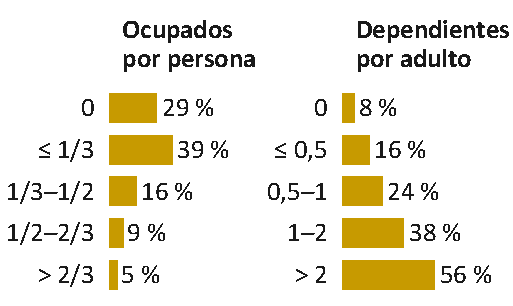
\includegraphics[width=\linewidth]{correlatos_pobreza}
    \column{0.38\textwidth}
      \footnotesize
      \textbf{Intuición.} Un modelo lineal suma efectos; un árbol corta en umbrales y
      combina variables.
      \begin{itemize}
        \item \textbf{No linealidad:} con más ocupados la pobreza sube de 29\,\% a 39\,\% y
          luego cae a 5\,\%.
        \item \textbf{Interacción:} el arriendo pesa distinto si la vivienda es propia o
          arrendada (la interacción más fuerte en un EBM).
        \item \textbf{Desbalance:} 20\,\% de pobres; el umbral se elige fuera de fold.
      \end{itemize}
  \end{columns}
  \takeaway{Esperamos que los métodos de árboles con muchas variables ganen a los lineales.}
  \fuente{Fuente: base de hogares de train (scripts/13\_figuras\_presentacion.R); views/tablas/nivel7/etapa15\_ebm\_importancia.csv.}
  \note{
    \textbf{Qué decir.} Antes de comparar, una predicción desde los datos. La pobreza no
    responde de forma lineal: con cero ocupados es menor que con un tercio, porque hay
    pensionados. Y las variables interactúan: pagar arriendo no significa lo mismo en una
    casa propia que en una arrendada. Eso favorece a los árboles, que cortan en umbrales y
    combinan variables sin que se las especifiquemos.\\[3pt]
    \textbf{Pregunta difícil: ¿no basta con interacciones en el Logit?} Se podrían
    agregar, pero habría que elegirlas a mano entre más de mil pares posibles; los árboles
    las buscan solos. El costo es la interpretabilidad.
  }
\end{frame}

%% ============================================================
\section{Comparación de algoritmos}
%% ============================================================
\begin{frame}{Cancha nivelada: mismas 48 variables, misma receta y misma validación}
  \centering\scriptsize\renewcommand{\arraystretch}{1.12}
  \begin{tabular}{@{}lllr@{}}
    \toprule
    Algoritmo & Búsqueda (validación cruzada de 5 folds) & Elegido & Configs. \\
    \midrule
    LPM y Logit & sin hiperparámetros & & 1 \\
    Elastic Net & grilla: penalización $10^{[-5,\,0]}$ $\times$ mezcla L1/L2 [0, 1] & 0,0002; 0,2 & 120 \\
    CART & grilla: complejidad $10^{[-5,\,-1]}$ $\times$ profundidad [3, 15] & $6\times10^{-5}$; 10 & 36 \\
    Naive Bayes & grilla: suavizado [0,5; 1,5] $\times$ Laplace [0, 3] & 0,5; 0 & 16 \\
    Random Forest & hipercubo: variables por corte [3, 25] $\times$ tamaño de hoja [5, 60] & 23; 24 & 15 \\
    XGBoost & hipercubo: árboles [200, 1000] $\times$ profundidad [3, 8] $\times$ tasa $10^{[-3,\,-1]}$ & 781; 6; 0,020 & 20 \\
    LightGBM & hipercubo de 7 hiperparámetros & ver apéndice & 50 \\
    \bottomrule
  \end{tabular}
  \vspace{0.25cm}

  \raggedright\small
  Todos usan la misma receta (imputación, dummies y escalado ajustados dentro de cada
  fold), el umbral elegido con predicciones fuera de fold y el mismo holdout del 20\,\%.
  \takeaway{Las diferencias de F1 reflejan el algoritmo, no los datos que recibe.}
  \fuente{Fuente: views/tablas/leaderboard\_interno.csv (columnas busqueda e hiperparametros).}
  \note{
    \textbf{Qué decir.} Para que la comparación sea justa, todos los algoritmos reciben
    las mismas 48 variables, el mismo preprocesamiento ajustado solo con los datos de
    entrenamiento de cada fold, y eligen hiperparámetros con validación cruzada de 5 folds.
    Grilla regular cuando hay 1 o 2 hiperparámetros, hipercubo latino cuando hay más.\\[3pt]
    \textbf{Pregunta difícil: ¿no tienen ventaja los que recibieron más configuraciones?}
    LightGBM probó 50 y XGBoost 20, pero XGBoost ya llegaba a 0,746 frente a 0,749: la
    ventaja de tuning es de 0,003. Elastic Net probó 120 y empata con el Logit sin tuning.
  }
\end{frame}

\begin{frame}{Con las mismas variables, el boosting gana y Naive Bayes queda 11 puntos atrás}
  \begin{columns}[c]
    \column{0.60\textwidth}
      \centering\scriptsize\renewcommand{\arraystretch}{1.1}
      \begin{tabular}{@{}lcccc@{}}
        \toprule
        Algoritmo & F1 CV & F1 holdout & Filtración & Subcob. \\
        \midrule
        \textbf{Boosting (LightGBM)} & \textbf{0,744} & \textbf{0,749} & 29,3\,\% & 20,4\,\% \\
        Boosting (XGBoost) & 0,740 & 0,746 & 29,6\,\% & 20,6\,\% \\
        Random Forest & 0,726 & 0,734 & 32,0\,\% & 20,2\,\% \\
        Elastic Net & 0,717 & 0,718 & 33,2\,\% & 22,4\,\% \\
        Logit & 0,717 & 0,718 & 32,7\,\% & 23,2\,\% \\
        CART & 0,697 & 0,701 & 34,3\,\% & 24,8\,\% \\
        LPM & 0,690 & 0,691 & 34,9\,\% & 26,3\,\% \\
        Naive Bayes & 0,643 & 0,640 & 44,0\,\% & 25,2\,\% \\
        \bottomrule
      \end{tabular}
    \column{0.38\textwidth}
      \footnotesize
      \textbf{Filtración} $=$ no pobres entre los atendidos ($1-$precisión).
      \textbf{Subcobertura} $=$ pobres excluidos ($1-$recall).
      \begin{itemize}
        \item El orden se repite en CV y en holdout: no es ruido de una partición.
        \item Los mejores ganan sobre todo en filtración.
        \item Naive Bayes supone variables independientes; aquí están muy correlacionadas.
      \end{itemize}
  \end{columns}
  \takeaway{Los dos más cercanos al ganador son Random Forest y Elastic Net (con Logit).}
  \fuente{Holdout de 32.993 hogares; umbral elegido con OOF. Fuente: views/tablas/comparacion\_algoritmos.csv; views/tablas/leaderboard\_interno.csv.}
  \note{
    \textbf{Qué decir.} Esta es la comparación de los siete algoritmos del curso con las
    mismas variables. El boosting queda primero y Naive Bayes último. El orden es el mismo
    en validación cruzada y en holdout. Los dos contendores más cercanos son Random Forest
    y Elastic Net, que empata con el Logit.\\[3pt]
    \textbf{Pregunta difícil: ¿son significativas estas diferencias?} Con 32.993 hogares,
    el efecto mínimo detectable en holdout está entre 0,0025 y 0,006 según el par: las
    brechas de 0,015 o más están claramente por encima; la de XGBoost frente a LightGBM, no.
  }
\end{frame}

\begin{frame}{Random Forest cubre igual que el boosting, pero filtra más}
  \begin{columns}[T]
    \column{0.50\textwidth}
      \centering\footnotesize
      \begin{tabular}{@{}lcc@{}}
        \toprule
        Holdout, 48 variables & Random Forest & XGBoost \\
        \midrule
        Recall (cobertura) & 0,798 & 0,794 \\
        Precisión & 0,680 & 0,704 \\
        No pobres incluidos & 2.483 & 2.206 \\
        Pobres excluidos & 1.332 & 1.358 \\
        F1 & 0,734 & 0,746 \\
        \bottomrule
      \end{tabular}
      \vspace{0.25cm}

      \begin{tabular}{@{}lcc@{}}
        \toprule
        Con variables de ingreso & F1 holdout & Brecha \\
        \midrule
        LightGBM (todas) & 0,781 & \\
        Random Forest (60 mejores) & 0,776 & $-0{,}005$ \\
        \bottomrule
      \end{tabular}
    \column{0.46\textwidth}
      \footnotesize
      \textbf{Intuición.} Random Forest promedia árboles profundos que aprenden lo mismo en
      paralelo; el boosting suma árboles pequeños que corrigen los errores de los
      anteriores, como los hogares cerca de la línea.
      \begin{itemize}
        \item Misma cobertura, pero 277 no pobres más incluidos: la brecha está en la
          precisión.
        \item Con las variables de ingreso la brecha baja de 0,012 a 0,005: con mejores
          variables, el algoritmo importa menos.
      \end{itemize}
  \end{columns}
  \takeaway{La ventaja del boosting está en la precisión: incluye menos no pobres.}
  \fuente{Fuente: views/tablas/leaderboard\_interno.csv; views/tablas/nivel7/etapa9\_candidatos.csv (Random Forest con las 60 variables de un algoritmo genético; no es cancha nivelada).}
  \note{
    \textbf{Qué decir.} Random Forest es el contendor más cercano. Cubre a los mismos
    pobres que el boosting, pero incluye 277 no pobres más. Una lectura: el bosque promedia
    árboles independientes, mientras el boosting agrega árboles enfocados en los errores
    que quedan, que están cerca de la línea. Con las variables de ingreso, la brecha se
    reduce a la mitad.\\[3pt]
    \textbf{Pregunta difícil: ¿la comparación del nivel 7 es justa?} No del todo: el bosque
    usó 60 variables y LightGBM todas. Por eso solo la usamos para mostrar que la brecha
    se achica, no para medirla.
  }
\end{frame}

\begin{frame}{Elastic Net empata con el Logit: la brecha con el boosting es por la linealidad}
  \begin{columns}[T]
    \column{0.48\textwidth}
      \footnotesize
      \textbf{Intuición.} Elastic Net penaliza coeficientes para evitar el sobreajuste. Con
      131.967 hogares y 48 variables no hay sobreajuste que evitar.
      \begin{itemize}
        \item La validación cruzada elige una penalización casi nula (0,0002).
        \item Mismo F1 en holdout que el Logit: 0,718.
        \item LPM (probabilidad lineal): 0,691, es decir 0,027 menos que el Logit.
      \end{itemize}
    \column{0.48\textwidth}
      \footnotesize
      \textbf{Lo que cuesta la linealidad frente al boosting}
      \begin{itemize}
        \item F1: 0,718 frente a 0,749 ($-0{,}031$).
        \item Subcobertura 22,4\,\% frente a 20,4\,\%: unos 130 pobres más excluidos en
          el holdout.
        \item A cambio, cada coeficiente se puede leer y auditar.
      \end{itemize}
  \end{columns}
  \takeaway{Regularizar no ayuda con muchos datos; lo que falta son umbrales e interacciones.}
  \fuente{Fuente: views/tablas/leaderboard\_interno.csv (n4\_elastic\_net, n3\_logit, n3\_lpm, n6\_lightgbm).}
  \note{
    \textbf{Qué decir.} El segundo contendor es Elastic Net. La validación cruzada elige
    casi no penalizar, porque con más de 130 mil hogares y 48 variables no hay sobreajuste.
    Por eso empata con el Logit. Lo que lo separa del boosting no es la regularización sino
    la forma funcional: no capta umbrales ni interacciones.\\[3pt]
    \textbf{Pregunta difícil: ¿cuántos pobres más excluye?} Con 6.605 pobres en el
    holdout, 2 puntos de subcobertura son unos 130 hogares (1.478 frente a 1.347
    excluidos).
  }
\end{frame}

\begin{frame}{Balancear las clases no mejora: solo mueve el umbral}
  \begin{columns}[c]
    \column{0.50\textwidth}
      \centering\footnotesize
      \begin{tabular}{@{}lcc@{}}
        \toprule
        XGBoost, 48 variables & F1 holdout & Umbral óptimo \\
        \midrule
        Sin balancear & 0,746 & 0,36 \\
        SMOTE & 0,745 & 0,34 \\
        Pesos de clase & 0,744 & 0,66 \\
        Submuestreo & 0,747 & 0,69 \\
        \bottomrule
      \end{tabular}
    \column{0.46\textwidth}
      \footnotesize
      \textbf{Intuición.} Balancear infla la probabilidad de ser pobre. Si después se elige
      el umbral que maximiza F1, ese umbral sube y deshace el cambio.
      \begin{itemize}
        \item Diferencias de F1 de 0,002 o menos, dentro del ruido.
        \item El umbral pasa de 0,36 a 0,66--0,69 con pesos o submuestreo.
      \end{itemize}
  \end{columns}
  \takeaway{Con el umbral elegido fuera de fold, el desbalance ya está resuelto.}
  \fuente{Fuente: views/tablas/leaderboard\_interno.csv (n4\_xgboost y n5\_*).}
  \note{
    \textbf{Qué decir.} Probamos las tres estrategias clásicas sobre el mejor algoritmo
    de ese nivel. Ninguna cambia el F1 más allá de 0,002. Lo que sí cambia es el umbral
    óptimo, porque el balanceo solo reescala las probabilidades.\\[3pt]
    \textbf{Pregunta difícil: ¿y si no se eligiera el umbral?} Con el umbral fijo en 0,5,
    esperaríamos que balancear sí ayudara, porque acerca las probabilidades al punto de
    corte (no lo medimos). Elegir el umbral es la forma directa de lograr lo mismo.
  }
\end{frame}

\begin{frame}{Cambiar las variables vale 9 veces más que cambiar el algoritmo}
  \begin{columns}[c]
    \column{0.66\textwidth}
      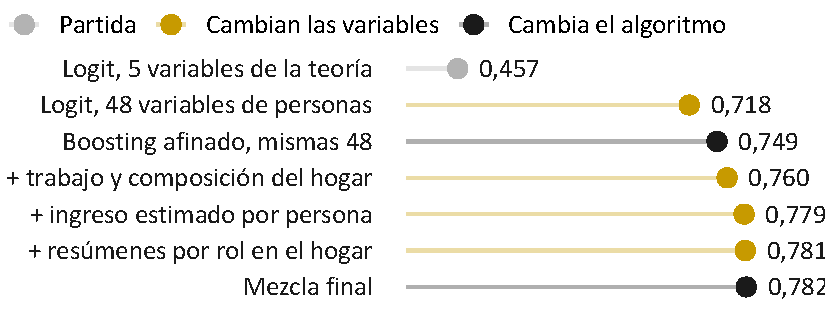
\includegraphics[width=\linewidth]{escalera_completa}
    \column{0.32\textwidth}
      \footnotesize
      \textbf{Suma de los saltos}
      \begin{itemize}
        \item \textcolor{andesaccent}{\textbf{Variables}}: $+0{,}292$.
        \item \textbf{Algoritmo}: $+0{,}032$.
      \end{itemize}
      La variable que más aportó predice el ingreso de cada persona con un modelo
      auxiliar y lo suma al hogar.
  \end{columns}
  \takeaway{La mejor inversión fue entender el hogar, no elegir el algoritmo.}
  \fuente{F1 en holdout. Fuente: views/tablas/leaderboard\_interno.csv y nivel7/ (ablacion\_etapa1, resumen\_etapa2, etapa6\_ablacion, etapa7\_a, etapa18\_resumen).}
  \note{
    \textbf{Qué decir.} Poniendo la comparación en perspectiva: toda la diferencia entre
    algoritmos que acabamos de ver suma 0,03 de F1. Construir variables desde las
    personas, y sobre todo predecir el ingreso de cada persona, sumó 0,29.\\[3pt]
    \textbf{Pregunta difícil: ¿no depende del orden de los pasos?} Sí, la descomposición
    es secuencial. Pero en cualquier orden el contraste es grande: con LightGBM fijo las
    variables nuevas suman 0,032, más que toda la diferencia entre Logit y boosting.
  }
\end{frame}

\begin{frame}{Con las variables de ingreso, todos los algoritmos convergen}
  \begin{columns}[c]
    \column{0.55\textwidth}
      \centering\scriptsize\renewcommand{\arraystretch}{1.1}
      \begin{tabular}{@{}lcc@{}}
        \toprule
        Base de 1.324 variables & F1 holdout & Corr.\ OOF \\
        \midrule
        \textbf{LightGBM} & \textbf{0,781} & 1 \\
        CatBoost & 0,779 & 0,994 \\
        AutoGluon (AutoML) & 0,777 & 0,990 \\
        RealMLP (red neuronal) & 0,775 & 0,984 \\
        TabM (red neuronal) & 0,767 & 0,977 \\
        \bottomrule
      \end{tabular}
    \column{0.43\textwidth}
      \footnotesize
      \textbf{Intuición.} Si todos predicen casi lo mismo, la información se agotó en las
      variables.
      \begin{itemize}
        \item Corr.\ OOF: correlación de sus predicciones fuera de fold con las de LightGBM; entre 0,98 y 0,99.
        \item AutoGluon sobre la base cruda, sin nuestras variables: 0,763.
        \item Mezclar los mejores suma una milésima (0,782).
      \end{itemize}
  \end{columns}
  \takeaway{El techo es común a todos: es de información, no de algoritmo.}
  \fuente{Fuente: views/tablas/nivel7/etapa7\_b.csv, etapa10\_candidatos.csv, etapa12\_resumen.csv, etapa18\_resumen.csv.}
  \note{
    \textbf{Qué decir.} Fuera de la lista del curso probamos CatBoost, redes neuronales
    tabulares y AutoML. Con nuestras variables todos quedan a menos de 0,015 de LightGBM y
    sus predicciones son casi idénticas. AutoGluon con la base cruda pierde 1,7 puntos: lo
    que le falta son nuestras variables, no capacidad de modelar.\\[3pt]
    \textbf{Pregunta difícil: ¿por qué gana LightGBM y no la red?} Con datos tabulares de
    este tamaño, los árboles con boosting suelen ganar a las redes; aquí la diferencia es de
    0,005, del orden del efecto mínimo detectable.
  }
\end{frame}

%% ============================================================
\section{Conclusión}
%% ============================================================
\begin{frame}{Más complejidad compra 6 puntos de F1 y protege más a los más pobres}
  \centering\footnotesize\renewcommand{\arraystretch}{1.12}
  \begin{tabular}{@{}lccc@{}}
    \toprule
    & Encuesta corta (Logit) & Logit completo & Mejor modelo \\
    \midrule
    Variables & 8 & 48 & 1.324 + auxiliares \\
    F1 holdout & 0,664 & 0,718 & 0,782 \\
    Subcobertura & 26,0\,\% & 23,2\,\% & 18,2\,\% \\
    Filtración & 39,8\,\% & 32,7\,\% & 25,1\,\% \\
    Excluidos en pobreza extrema & 16,1\,\% & 14,8\,\% & 11,2\,\% \\
    Interpretación & coeficientes & coeficientes & importancia y curvas \\
    Costo de recolección & bajo & medio & alto (módulo laboral) \\
    \bottomrule
  \end{tabular}
  \vspace{0.2cm}

  \raggedright\footnotesize
  Pobreza extrema: ingreso menor a la mitad de la línea, como porcentaje de los pobres excluidos.
  \takeaway{La complejidad se justifica por a quién deja de excluir, no por el F1 en sí.}
  \fuente{Holdout, umbral elegido con OOF. Fuente: views/tablas/nivel7/etapa15\_pesos\_bienestar.csv (mejor modelo: mezcla sin el modelo limpio).}
  \note{
    \textbf{Qué decir.} El trade-off concreto: pasar de 8 preguntas a un Logit completo y
    luego al mejor modelo baja la subcobertura de 26 a 18\,\% y la filtración de 40 a
    25\,\%. Y no solo excluye menos: los que excluye están más cerca de la línea.\\[3pt]
    \textbf{Pregunta difícil: ¿el mejor modelo es interpretable?} No como un Logit, pero
    sus decisiones se explican con dos cosas: ingreso predicho y vivienda. Un EBM llega a
    0,777 con curvas legibles, por si la agencia exige transparencia.
  }
\end{frame}

\begin{frame}{¿El modelo con más score en Kaggle? No necesariamente}
  \small
  \textbf{Lo que recomendaríamos a una agencia}
  \begin{enumerate}
    \item \textbf{Elegir por el costo de los errores, no por F1:} el F1 supone que excluir y
      filtrar cuestan igual; una agencia puede preferir más cobertura.
    \item \textbf{LightGBM solo, no la mezcla:} rinde igual (diferencia de milésimas) y es más
      simple de mantener y auditar.
    \item \textbf{Si exige transparencia:} un EBM (0,777) o un Logit (0,718) con el mismo
      módulo laboral, aceptando más subcobertura.
    \item \textbf{Si solo hay encuesta corta:} el Logit de 8 preguntas como filtro, con un
      umbral más bajo y verificación posterior.
  \end{enumerate}
  \takeaway{La mejor decisión depende de qué se puede medir y de cuánto cuesta excluir a un pobre.}
  \fuente{Fuente: views/tablas/nivel7/etapa15\_resumen.csv (EBM); views/tablas/leaderboard\_interno.csv; views/tablas/nivel7/etapa18\_resumen.csv.}
  \note{
    \textbf{Qué decir.} No necesariamente el de mayor Kaggle. La diferencia entre la
    mezcla y LightGBM solo es de milésimas, así que recomendamos el más simple. Si la
    agencia necesita explicar cada decisión, un EBM pierde medio punto. Y si solo puede
    pagar una encuesta corta, debe compensar con un umbral más bajo y verificación.\\[3pt]
    \textbf{Pregunta difícil: ¿por qué no recomiendan directamente el Logit, que es
    transparente?} Porque excluye a 5 puntos más de pobres y más de ellos en pobreza
    extrema; esa es una pérdida de bienestar que hay que poner en la balanza.
  }
\end{frame}

%% ============================================================
%% Apéndice
%% ============================================================
\appendix
\diapositivaglosario

\begin{frame}{Apéndice: hiperparámetros del LightGBM ganador}
  \centering\footnotesize\renewcommand{\arraystretch}{1.12}
  \begin{tabular}{@{}llll@{}}
    \toprule
    Hiperparámetro & Rango explorado & Elegido & Lectura \\
    \midrule
    Número de árboles & [200, 2000] & 1.852 & muchos árboles \\
    Tasa de aprendizaje & $10^{[-3,\,-0{,}7]}$ & 0,011 & pasos pequeños \\
    Profundidad máxima & [3, 12] & 12 (31 hojas) & árboles medianos \\
    Mínimo de hogares por hoja & [10, 200] & 171 & no memoriza casos \\
    Variables por corte & [0,2; 1] & 0,82 & algo de azar \\
    Hogares por árbol & [0,5; 1] & 0,70 & algo de azar \\
    Ganancia mínima para cortar & $10^{[-10,\,1]}$ & $7\times10^{-10}$ & sin restricción \\
    \bottomrule
  \end{tabular}
  \fuente{Hipercubo latino de 50 configuraciones, validación cruzada de 5 folds sobre las 48 variables. Fuente: views/tablas/leaderboard\_interno.csv (n6\_lightgbm).}
  \note{Respaldo: la configuración que se reutilizó en todo el nivel 7.}
\end{frame}

\begin{frame}{Apéndice: en CV repetida ninguna alternativa mejora de forma detectable}
  \centering\scriptsize
  \begin{tabular}{@{}lccc@{}}
    \toprule
    Candidato & F1 CV repetida (EE) & $\Delta$ vs.\ LightGBM [IC 95\,\%] & F1 holdout [IC 95\,\%] \\
    \midrule
    LightGBM base & 0,7752 (0,0008) & & 0,7806 [0,7731; 0,7885] \\
    + redes (mezcla sin limpio) & 0,7758 (0,0008) & $+0{,}0006$ [$-0{,}0001$; $+0{,}0013$] & 0,7820 [0,7743; 0,7897] \\
    \textbf{+ redes + limpio (final)} & \textbf{0,7759 (0,0008)} & $+0{,}0007$ [$+0{,}0002$; $+0{,}0012$] & 0,7817 [0,7742; 0,7894] \\
    CatBoost & 0,7722 (0,0007) & $-0{,}0030$ [$-0{,}0042$; $-0{,}0018$] & 0,7786 [0,7707; 0,7864] \\
    Rediseño desde cero & 0,7478 (0,0008) & $-0{,}0274$ [$-0{,}0289$; $-0{,}0260$] & 0,7499 [0,7420; 0,7581] \\
    \bottomrule
  \end{tabular}
  \fuente{IC pareados ingenuos (15 pares). Con la corrección de Nadeau y Bengio el IC del modelo final es [$-0{,}0004$; $+0{,}0017$]. Fuente: views/tablas/nivel7/etapa16\_fase1\_resumen.csv, etapa18\_resumen.csv.}
  \note{Respaldo: CatBoost pierde con un IC que excluye cero; la mezcla gana por milésimas.}
\end{frame}

\end{document}
